
\documentclass[compress]{beamer}

%\usepackage{beamerthemesplit}
\usepackage{xmpmulti}

\definecolor{green}{rgb}{0,.3,0}

\usepackage{graphicx,float,wrapfig, bbm}
\usepackage{amsfonts, bbold, comment}
\usepackage{mdwlist}
\usepackage{listings}
\usepackage{environ}
\usepackage{subfigure}
\usepackage{rotating}
\usepackage{algorithmic}
\usepackage{algorithm}
\usepackage{overpic}
\usepackage{qtree}
\usepackage{mathtools}

\usepackage{multirow}

\usetheme[bullet=circle,                     % Use circles instead of squares for bullets.
          titleline=true,                    % Show a line below the frame title.
          showdate=true,                     % show the date on the title page
          alternativetitlepage=true,         % Use the fancy title page.
          titlepagelogo=general_figures/culogo,              % Logo for the first page.
          % Logo for the header on first page.
          headerlogo=general_figures/boulder_cs,
          ]{UCBoulder}

\usecolortheme{ucdblack}

%\useoutertheme{infolines}
%\usetheme{Boadilla}
%\usetheme{Singapore}
% \usecolortheme{umd}
\title{Big Data Analysis with Topic Models: Human Interaction, Streaming Computation, and Social Science Applications}
\author{Jordan Boyd-Graber}
\date{27. January 2017}

\newcommand{\fsi}[2]{
\begin{frame}[plain]
\vspace*{-1pt}
\makebox[\linewidth]{\includegraphics[width=\paperwidth]{#1}}
\begin{center}
#2
\end{center}
\end{frame}
}

\newcommand{\gfxtp}[2]{
\begin{center}
	\includegraphics[width=#2\linewidth]{teaparty/figures/#1}
\end{center}
}

\newcommand{\gfxag}[2]{\begin{center}
    \includegraphics[width=#2\linewidth]{onlineag/#1}
\end{center}
}

\newcommand{\subtwo}[2]{_{#1, #2}}
\newcommand{\subthree}[3]{_{#1, #2, #3}}


\newcommand{\explain}[2]{\underbrace{#2}_{\mbox{\footnotesize{#1}}}}
\newcommand{\dir}[1]{\mbox{Dir}(#1)}
\newcommand{\mult}[1]{\mbox{Mult}( #1)}
\newcommand{\Beta}[1]{\mbox{Beta}( #1)}
\newcommand{\G}[1]{\Gamma \left( \textstyle #1 \right)}
\newcommand{\LG}[1]{\log \Gamma \left( \textstyle #1 \right)}
\newcommand{\WN}[0]{\textsc{WordNet}}
\newcommand{\itmspace}[0]{\hspace{2cm}}
\newcommand{\abr}[1]{\textsc{#1}}
\newcommand{\lda}[0]{\abr{lda}}
\newcommand{\slda}[0]{\abr{slda}}

\newcommand{\digam}[1]{\Psi \left( \textstyle #1 \right) }
\newcommand{\ddigam}[1]{\Psi' \left( \textstyle #1 \right) }
\newcommand{\e}[2]{\mathbb{E}_{#1}\left[ #2 \right] }
\newcommand{\ind}[1]{\mathbb{I}\left[ #1 \right] }
\newcommand{\ex}[1]{\mbox{exp}\left\{ #1\right\} }
\newcommand{\D}[2]{\frac{\partial #1}{\partial #2}}
\newcommand{\elbo}{\mathcal{L}}


\newcommand{\citename}[1]{\emph{#1} }
\newcommand{\bm}[1]{\mbox{\boldmath$#1$}}
\newcommand{\Dir}{\mathrm{Dir}}
\newcommand{\Mult}{\mathrm{Mult}}
\newcommand{\g}[1]{\Gamma \left( #1 \right)}
\newcommand{\paragraph}[1]{ \vskip 1cm {\bf \large #1}}

\NewEnviron{smalign}{
\vspace{-.6cm}
\begin{small}
\begin{align}
  \BODY
\end{align}
\end{small}
\vspace{-.6cm}
}


\providecommand{\graphscale}{0.6}

\newcommand{\danquote}[1]{

\begin{flushright}
\begin{overpic}[width=5.5cm,tics=10]{general_figures/speech_bubble}
	\put(10,30) { \parbox{4cm}{#1 }}
\end{overpic}

\includegraphics[width=1.5cm]{general_figures/milkman_dan}
\end{flushright}
}


% \AtBeginSection[] % "Beamer, do the following at the start of every section"
% { \begin{frame}

% \frametitle{Outline} % make a frame titled "Outline"
% \tableofcontents[currentsection] % show TOC and highlight current section
% \end{frame} }

\lstset{language=Python}

\DeclareMathSymbol{\R}{\mathbin}{AMSb}{"52}

\setbeamertemplate{footline}{}

\begin{document}

% this prints title, author etc. info from above

\frame{\titlepage}



\begin{frame}
\frametitle{The Challenge of Big Data}

\begin{columns}

\column{.5\linewidth}

Every second \dots
\begin{itemize}
  \item 600 new blog posts appear
  \item 34,000 tweets are tweeted
  \item 30 GB of data uploaded to Facebook
\end{itemize}
\pause

\begin{block}{Unstructured}
  No XML, no semantic web, no annotation.  Often just raw text.
\end{block}

\column{.5\linewidth}

\only<3->{
Common task: what's going on in this dataset.
\begin{itemize}
   \item Intelligence analysts
   \item Brand monitoring
   \item Journalists
   \item Humanists
\end{itemize}
}
\only<4>{
\centering
Common solution: topic models
}

\end{columns}

\end{frame}

\begin{frame}

\begin{center}
\frametitle{Topic Models as a Black Box}
From an \textbf<1>{input corpus} and number of topics \textbf<1>{$K$} $\rightarrow$ \textbf<2>{words to topics} \\
\only<1>{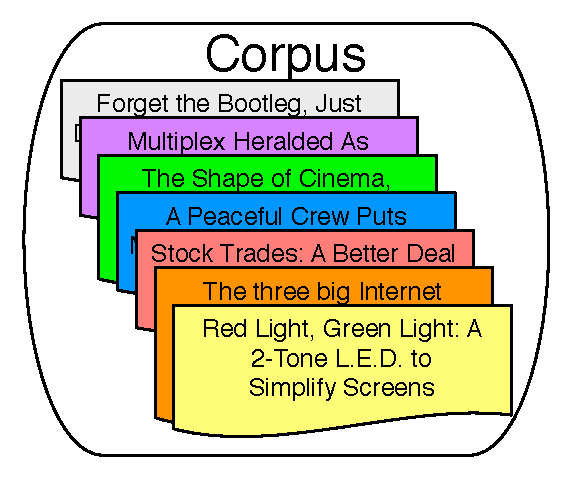
\includegraphics[width=0.6\linewidth]{reading_tea_leaves/figures/heldout_0} }
\only<2>{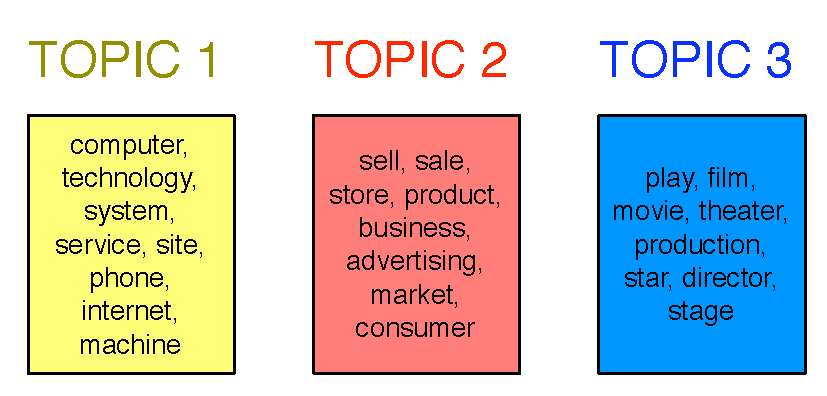
\includegraphics[width=0.9\linewidth]{reading_tea_leaves/figures/nyt_topics_wide}}
\only<3>{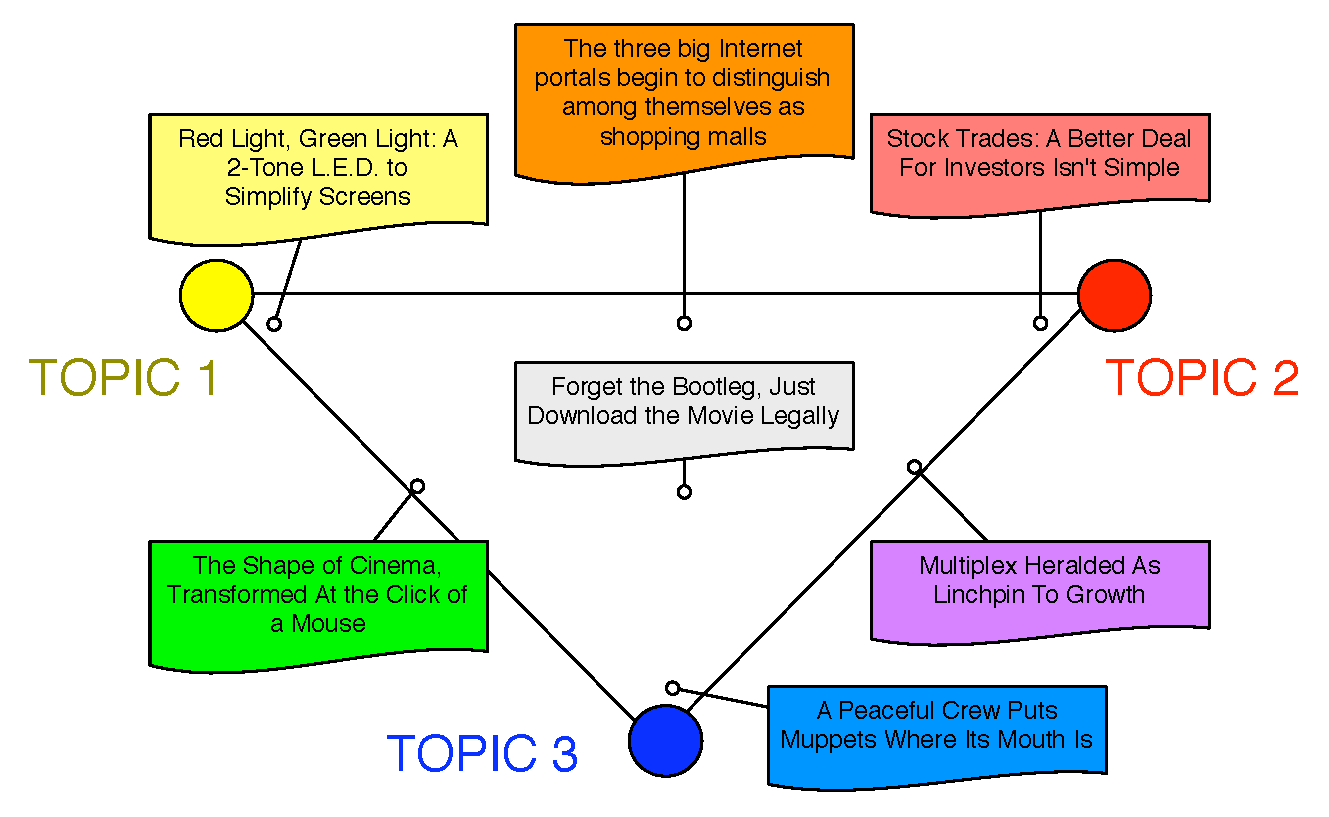
\includegraphics[width=0.9\linewidth]{topic_models/nyt_documents}}
\end{center}

\end{frame}




\frame{
  \frametitle{Word Intrusion}

  \begin{enumerate}
    \item Take the highest probability words from a topic

      \begin{block}{Original Topic}
        dog, cat, horse, pig, cow
      \end{block}
\pause
    \item Take a high-probability word from another topic and add it
      \begin{block}{Topic with Intruder}
        dog, cat, \alert<2->{apple}, horse, pig, cow
      \end{block}
\pause
     \item We ask users to find the word that doesn't belong
  \end{enumerate}
\begin{block}{Hypothesis}
If the topics are interpretable, users will consistently choose true intruder
\end{block}
}


\frame{
\frametitle{Word Intrusion: Which Topics are Interpretable?}
  \begin{block}{New York Times, 50 Topics}
    \begin{center}
      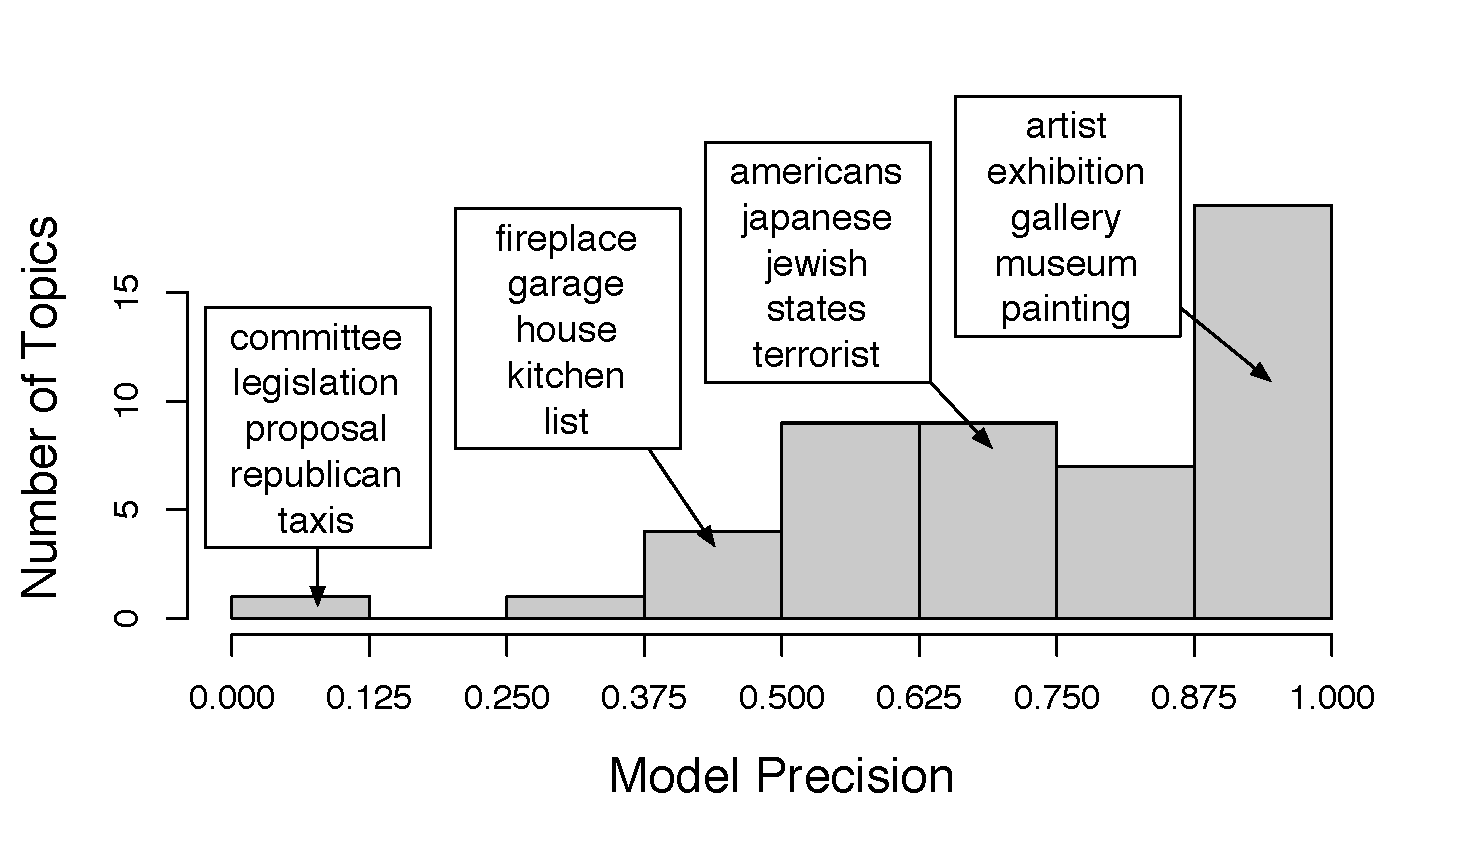
\includegraphics[width=0.8\linewidth]{reading_tea_leaves/figures/topic_precision}
    \end{center}
  \end{block}
  \begin{center}
    Model Precision: percentage of correct intruders found
  \end{center}
}

\frame{

\frametitle{Interpretability and Likelihood}

\begin{center}
\only<1>{Model Precision on New York Times}
\end{center}

\begin{columns}
\column{.84\linewidth}
\begin{flushright}
  \only<1>{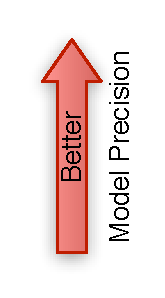
\includegraphics[scale=\graphscale]{reading_tea_leaves/tasks/mp}}
  \only<1>{
\includegraphics[scale=\graphscale]{reading_tea_leaves/tasks/mp_y}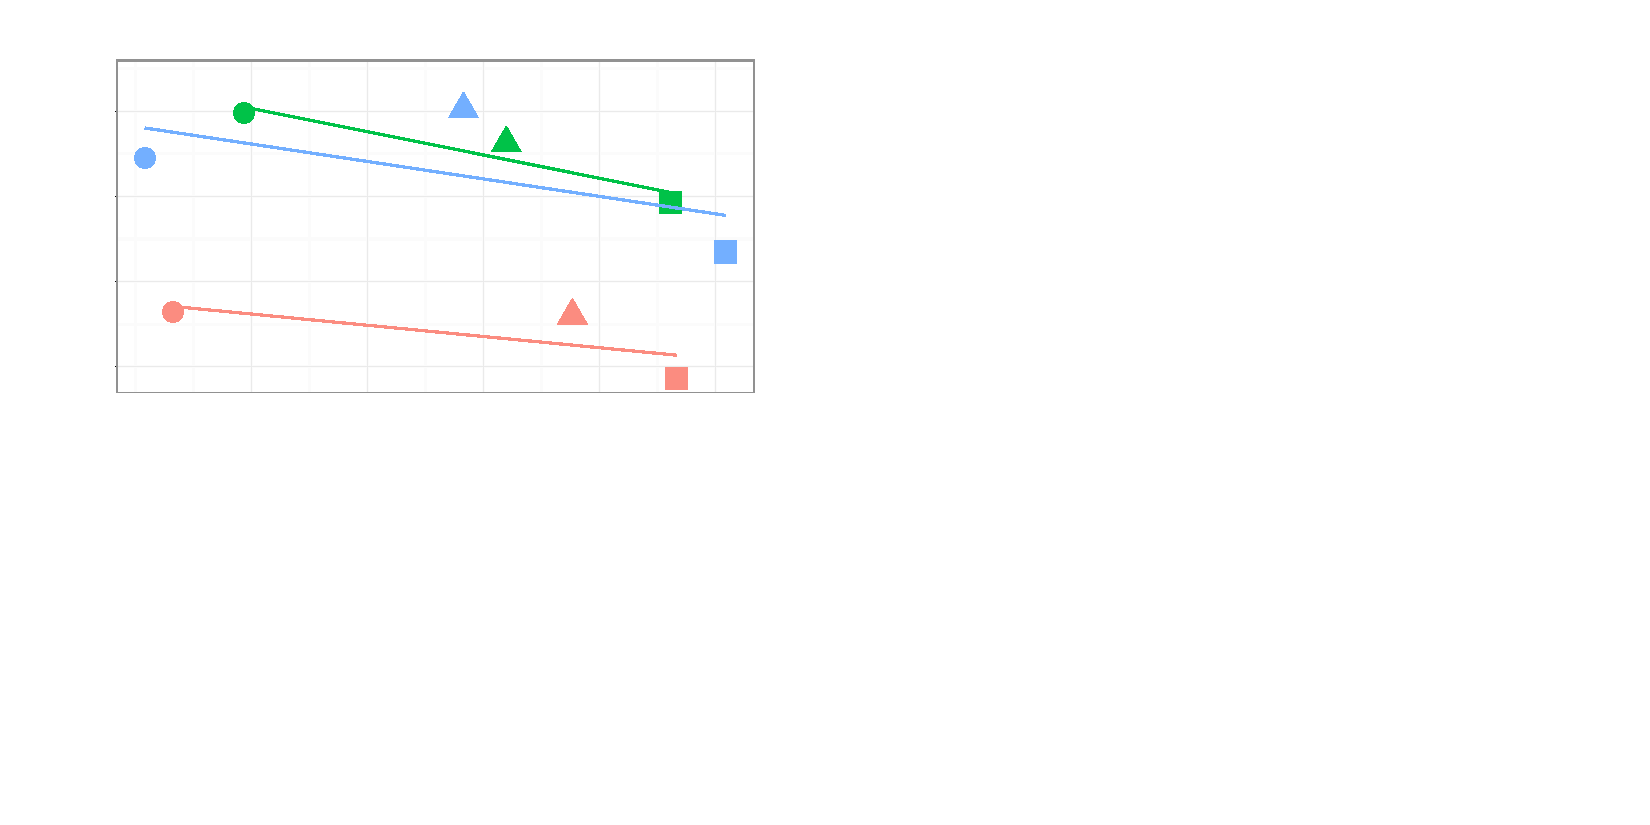
\includegraphics[scale=\graphscale]{reading_tea_leaves/tasks/nyt_mp}\\}
  \only<1>{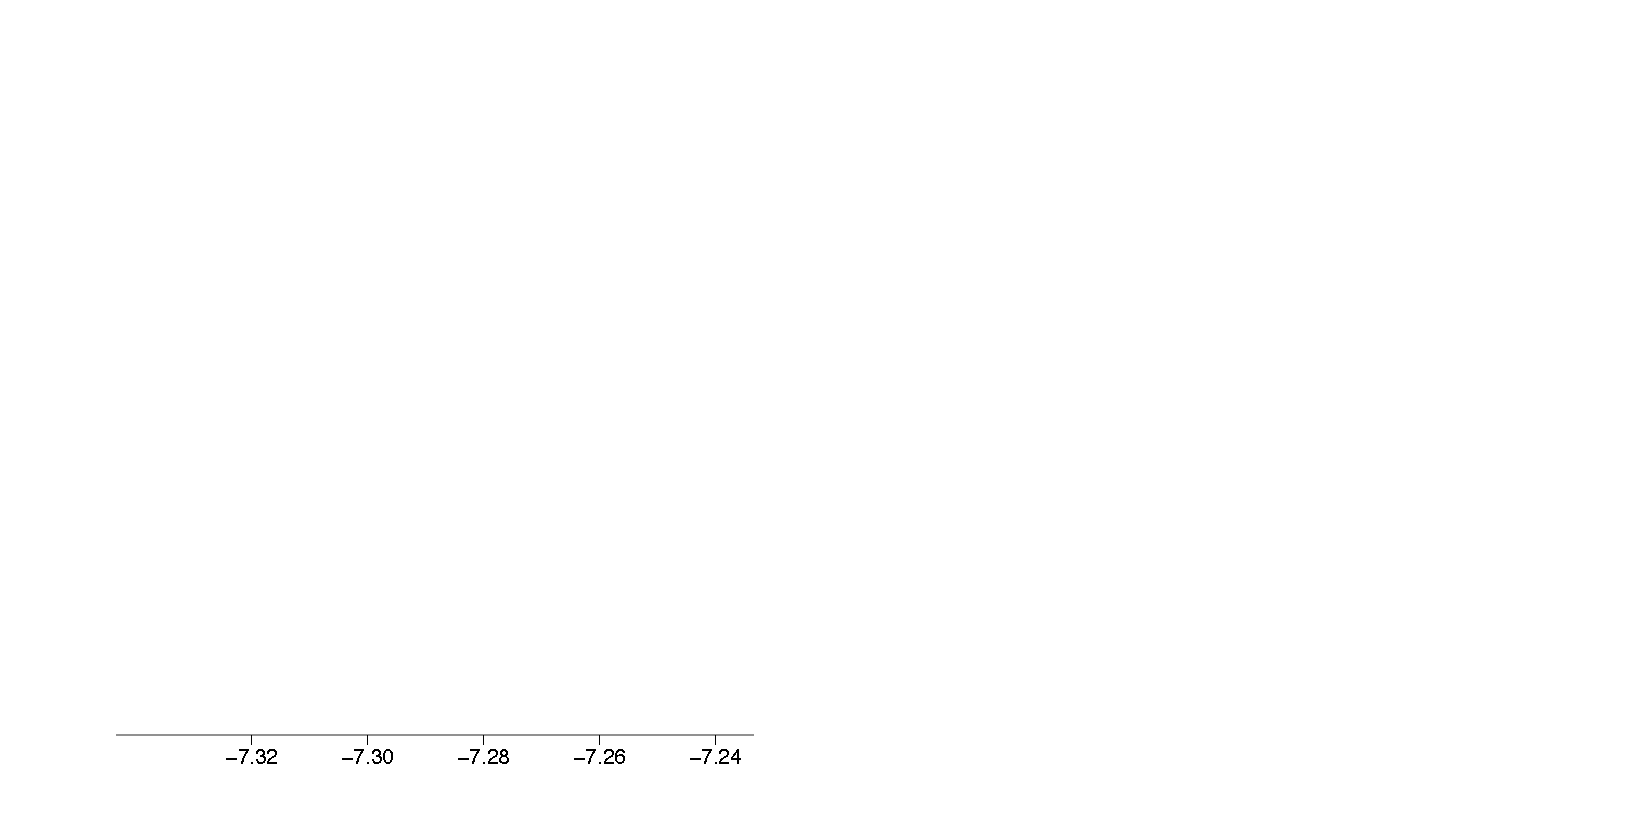
\includegraphics[scale=\graphscale]{reading_tea_leaves/tasks/nyt_x}}

\end{flushright}
\column{.15\linewidth}
  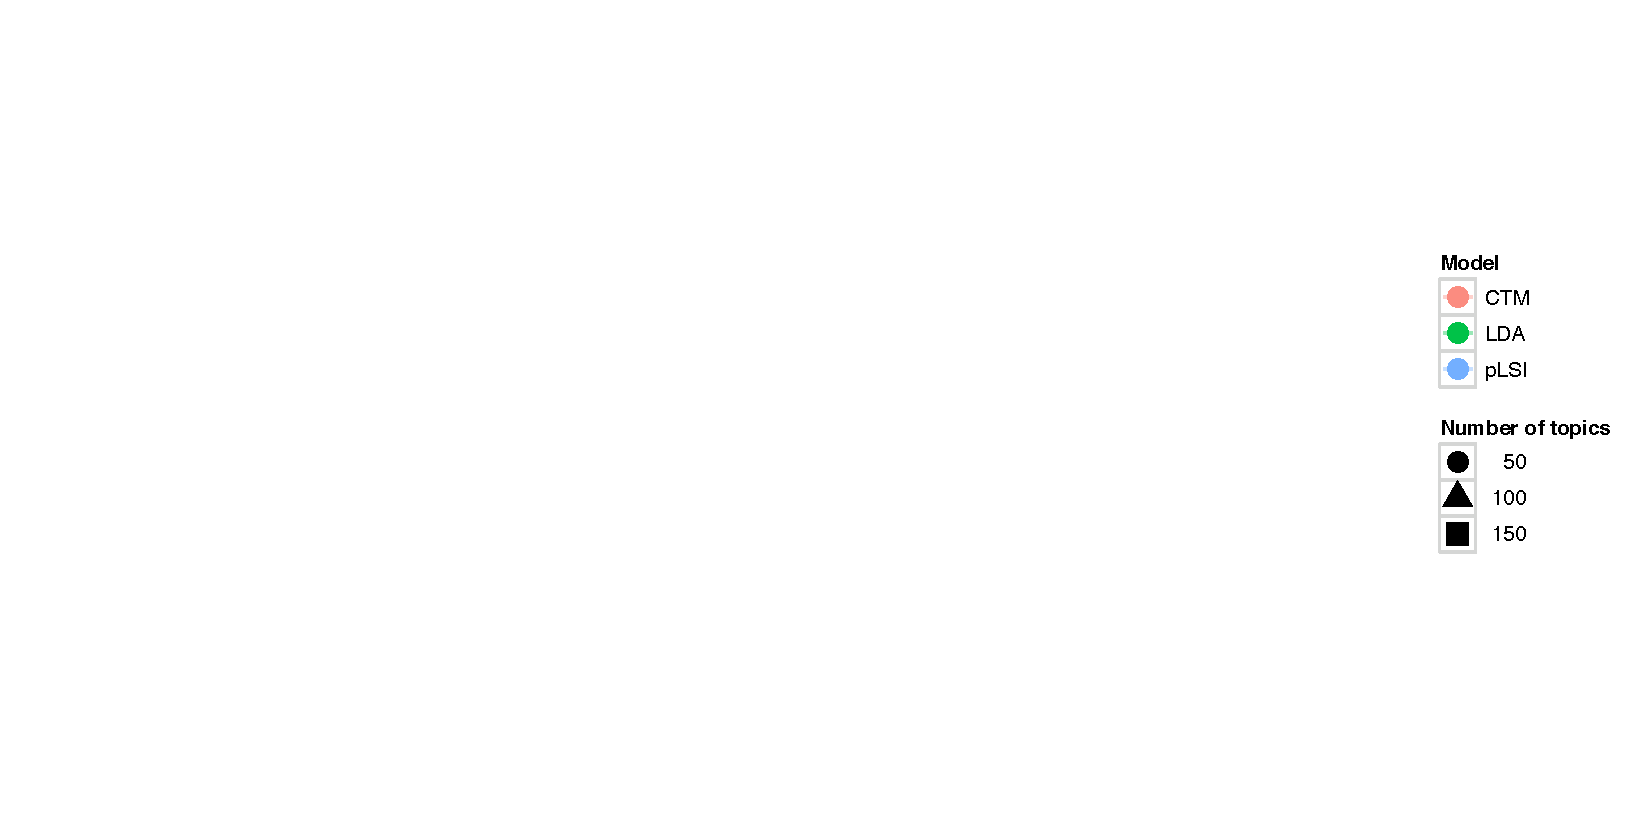
\includegraphics[scale=\graphscale]{reading_tea_leaves/tasks/legend}
\end{columns}
\vspace{-0.75cm}
\begin{center}
  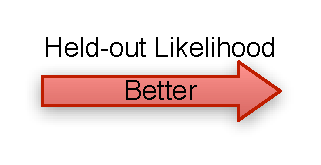
\includegraphics[scale=\graphscale]{reading_tea_leaves/tasks/held-out} \\
\only<1> {within a model, higher likelihood $\not =$ higher interpretability}
\end{center}
}



\frame{

\begin{columns}

\column{.5\linewidth}

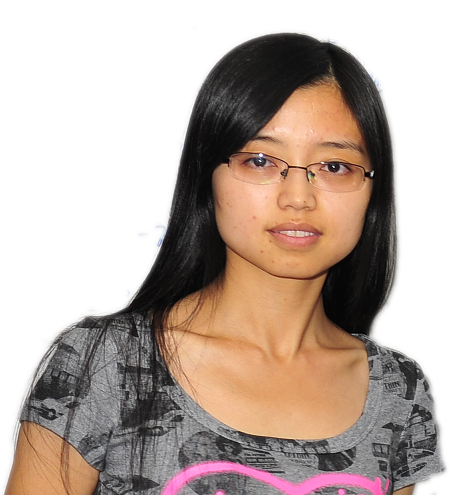
\includegraphics[width=.8\linewidth]{general_figures/yuening}

\column{.5\linewidth}

\begin{block}{Interactive Topic Modeling}
Yuening Hu, Jordan Boyd-Graber, Brianna Satinoff, and Alison Smith. Interactive Topic Modeling. Machine Learning, 2014.
\end{block}

\end{columns}

}



\providecommand{\tb}[1]{\parbox{0.8\linewidth}{ \tiny{ #1 }} \vspace{.2cm} }

\frame{

\vspace{-1cm}

\begin{columns}

\column{.5\linewidth}

\begin{tabular}{l*{2}{c}r}
	Topic & Before \\
\hline

\alert<2>{{\bf 1}} & \tb{ \alert<2>{election, yeltsin, russian, political, party, democratic, russia,
  president, democracy, boris, country, south, years, month, government, vote,
  since, leader, presidential, military} } \\

2 & \tb{new, york, city, state, mayor, budget, giuliani, council, cuomo, gov,
  plan, year, rudolph, dinkins, lead, need, governor, legislature, pataki,
  david} \\

3 & \tb{nuclear, arms, weapon, defense, treaty, missile, world, unite, yet,
  soviet, lead, secretary, would, control, korea, intelligence, test, nation,
  country, testing} \\

4 & \tb{president, bush, administration, clinton, american, force, reagan, war,
  unite, lead, economic, iraq, congress, america, iraqi, policy, aid,
  international, military, see} \\

& \vdots \\

\alert<2>{{\bf 20}} & \tb{\alert<2>{soviet, lead, gorbachev, union, west, mikhail, reform, change, europe,
  leaders, poland, communist, know, old, right, human, washington, western,
  bring, party} }\\

\end{tabular}

\column{.5\linewidth}

\only<3> {

	\begin{block}{Suggestion}
	\emph{boris, communist, gorbachev, mikhail, russia,
  russian, soviet, union, yeltsin }
	\end{block}

}

\only<4-> {

\begin{tabular}{l*{2}{c}r}
	Topic & After \\
\hline

\alert<5>{{\bf 1}} & \alert<5>{\tb{election, democratic, south, country, president, party, africa, lead,
  even, democracy, leader, presidential, week, politics, minister, percent,
  voter, last, month, years} } \\

\alert<6>{2} & \tb{new, york, city, state, mayor, budget, council, giuliani, gov, cuomo,
  year, rudolph, dinkins, legislature, plan, david, governor, pataki, need, cut}
\\

\alert<6>{3} & \tb{nuclear, arms, weapon, treaty, defense, war, missile, may, come, test,
  american, world, would, need, lead, get, join, yet, clinton, nation} \\

\alert<6>{4} & \tb{president, administration, bush, clinton, war, unite, force, reagan,
  american, america, make, nation, military, iraq, iraqi, troops, international,
  country, yesterday, plan} \\

   & \vdots \\

\alert<4>{ {\bf 20} } & \alert<4> {\tb{soviet, union, economic, reform, yeltsin, russian, lead, russia,
  gorbachev, leaders, west, president, boris, moscow, europe, poland, mikhail,
  communist, power, relations} } \\

\end{tabular}

}

\end{columns}

}


\providecommand{\blue}[1]{{\color{blue}{#1}}}
\providecommand{\red}[1]{{\color{red}{#1}}}
\providecommand{\green}[1]{{\color{green}{#1}}}

\begin{frame}

\frametitle{Example: Negative Constraint}

\begin{columns}

\column{.4\linewidth}

\begin{tabular}{l*{2}{c}r}
	Topic & Words \\
\hline

{\bf 318} & \tb{\red{bladder}, sci, \blue{spinal\_cord}, \blue{spinal\_cord\_injury}, \blue{spinal}, \red{urinary}, \red{urinary\_tract}, \red{urothelial},\blue{injury}, \blue{motor}, \blue{recovery}, \blue{reflex}, \blue{cervical}, \red{urothelium}, \blue{functional\_recovery}} \\

\end{tabular}

\column{.1\linewidth}

\column{.4\linewidth}

\only<3->{
\begin{tabular}{l*{2}{c}r}
	Topic & Words \\
\hline

{\bf 318} & \tb{sci, \blue{spinal\_cord}, \blue{spinal\_cord\_injury}, \blue{spinal}, \blue{injury}, \blue{recovery}, \blue{motor}, \blue{reflex}, \red{urothelial}, \green{injured}, \blue{functional\_recovery}, \green{plasticity}, \green{locomotor}, \blue{cervical}, \green{locomotion}}\\

\end{tabular}
}

\end{columns}

\only<2->{
\begin{block}{Negative Constraint}
  spinal\_cord, bladder
\end{block}

}

\end{frame}



\frame{

\begin{columns}

\column{.5\linewidth}

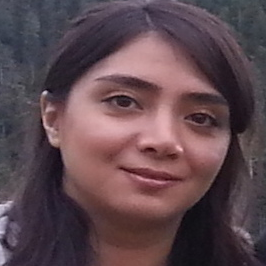
\includegraphics[width=.8\linewidth]{general_figures/forough}

\column{.5\linewidth}

\begin{block}{ALTO: Active Learning with Topic Overviews for Speeding Label Induction and Document Labeling}
Forough Poursabzi-Sangdeh, Jordan Boyd-Graber, Leah Findlater, and Kevin Seppi.  Association for Computational Linguistics, 2016.
\end{block}

\end{columns}

}

\fsi{interactive_topic_models/messy-desk}{Many Documents}

\fsi{interactive_topic_models/file-cabinet}{Sort into Categories}

\begin{frame}{Evaluation}

  \begin{itemize}
    \item User study
    \item 40 minutes
    \item Sort documents into categories
    \item What information / interface \alert<2>{helps best}
      \pause
      \pause
      \begin{itemize}
        \item Train a classifier on human examples
          \only<4->{\alert<4>{(don't tell them how many labels)}}
        \item Compare classifier labels to expert judgements
          \only<5->{\alert<5>{(purity)}}
\only<5>{
\begin{equation}
\mbox{purity}(\mathbf{U},\mathbf{G}) = \frac{1}{N}\sum\limits_{l} \max\limits_{j}|U_l \cap G_j|,
\end{equation}
}
      \end{itemize}
  \end{itemize}

\end{frame}

\begin{frame}{Which is more Useful?}

\only<1>{
  \begin{center}
    Who should drive?
  \end{center}
}


\only<2->{
\begin{columns}
  \column{.5\linewidth}
    \begin{block}{Active Learning}
      \begin{center}
        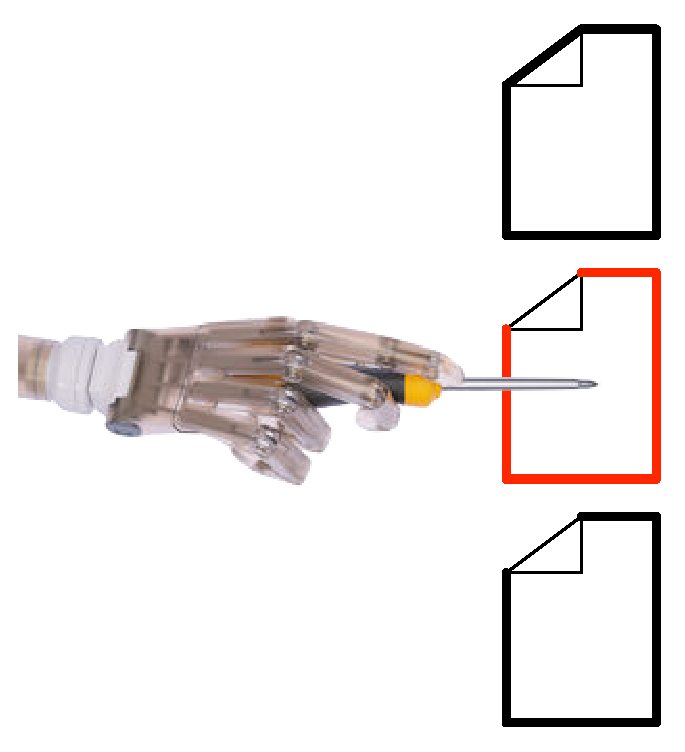
\includegraphics[width=.85\linewidth]{interactive_topic_models/active_learning}
      \end{center}
    \end{block}
  \column{.5\linewidth}
  \pause
    \begin{block}{Topic Models}
      \begin{center}
        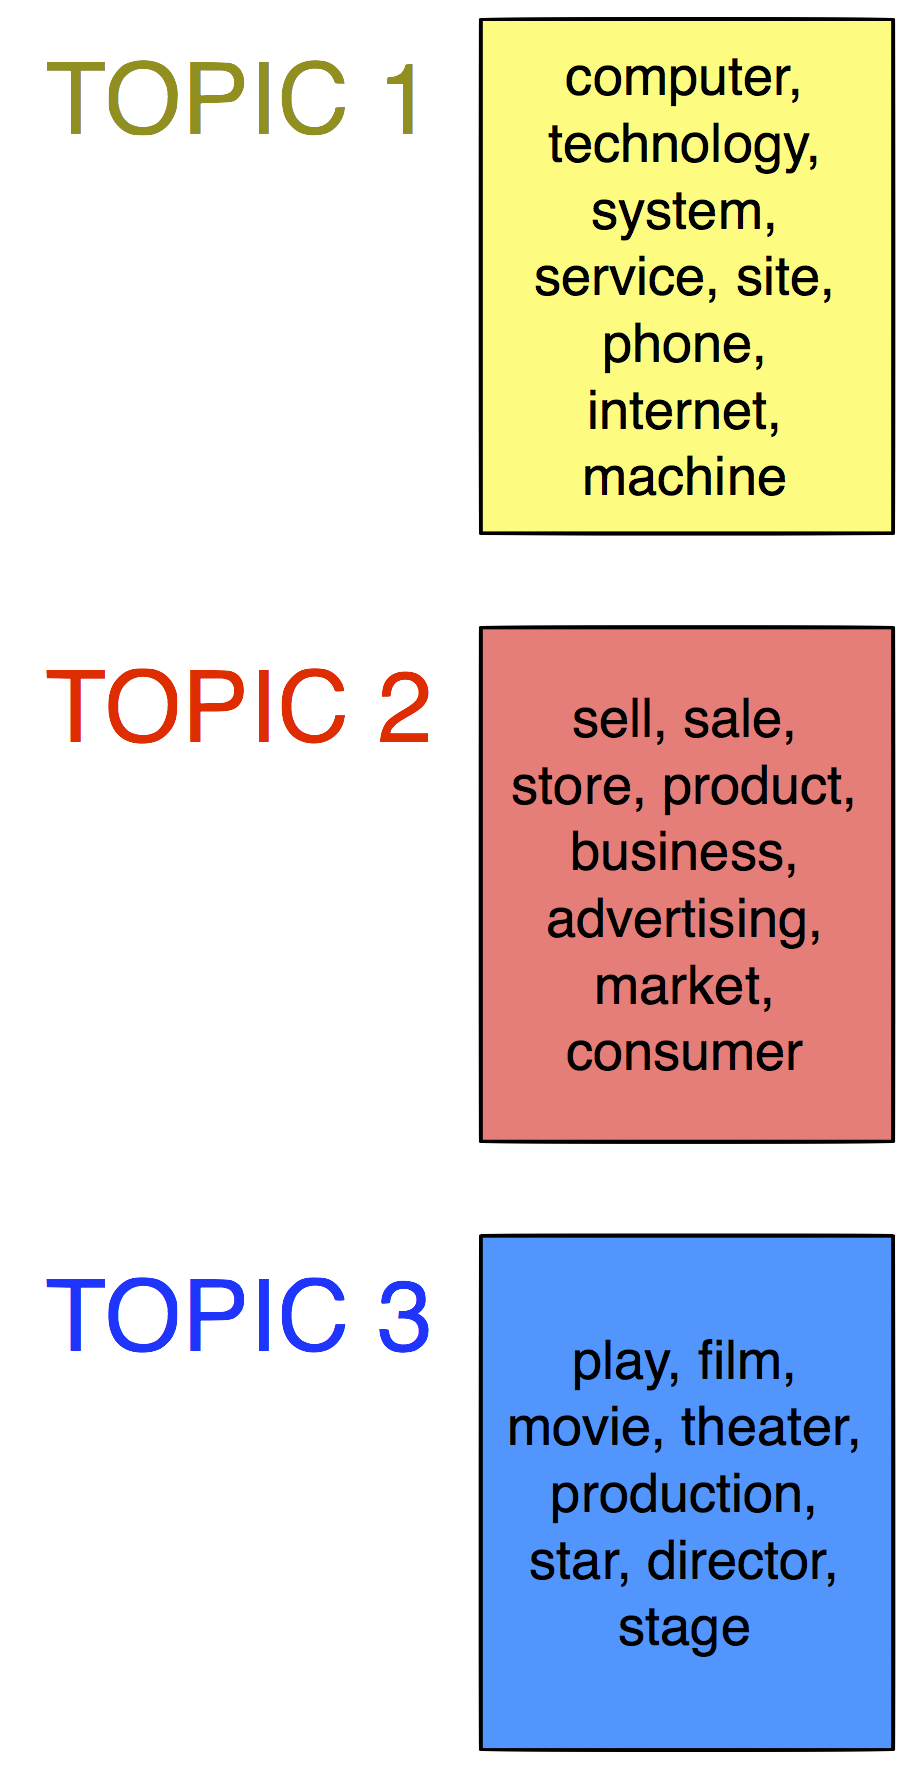
\includegraphics[width=.475\linewidth]{interactive_topic_models/nyt_topics}
      \end{center}

    \end{block}


\end{columns}
}

\end{frame}

\fsi{interactive_topic_models/alto_interface}{}
\fsi{interactive_topic_models/alto_interface_highlight}{Direct users
  to document}



\fsi{interactive_topic_models/alto/user_talk_1}{ Active learning if time is short}
\fsi{interactive_topic_models/alto/user_talk_2}{ Better than status quo}
\fsi{interactive_topic_models/alto/user_talk_3}{ Active learning can
  help topic models }
\fsi{interactive_topic_models/alto/user_talk_4}{ Topic models help
  users understand the collection }
\fsi{interactive_topic_models/alto/user_talk_4}{ Moral: machines and
  humans together (if you let them) }



\frame{
  \frametitle{Ongoing and Future Work}

  \begin{itemize}
        \item Embedding interactivity in applications
    \item Visualizations to measure machine learning explainability
    \item Using morphology in infinite representations
    \item Multilingual analysis
    \end{itemize}
}

\frame{
  \frametitle{But wait, there's more!}

\begin{columns}

  \column{.5\linewidth}
    \begin{block}{Question Answering}
    \centering
        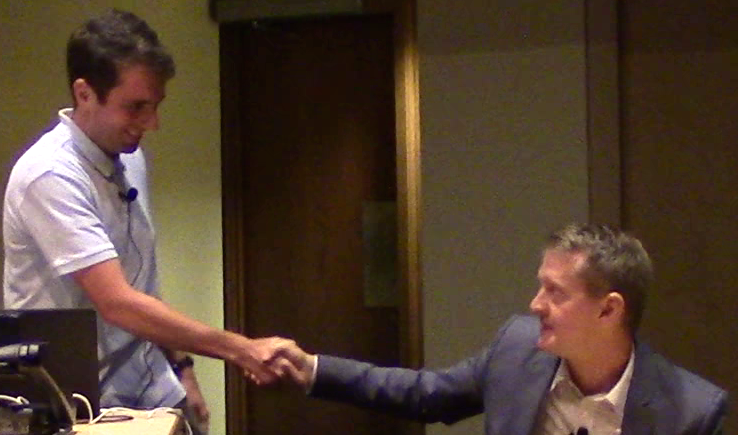
\includegraphics[width=0.5\linewidth]{qb/jennings_handshake} \\
     \small
       \cite{iyyer-15,He:Boyd-Graber:Daume-III-2016}
    \end{block}


    \begin{block}{Machine Translation}
      \begin{center}
        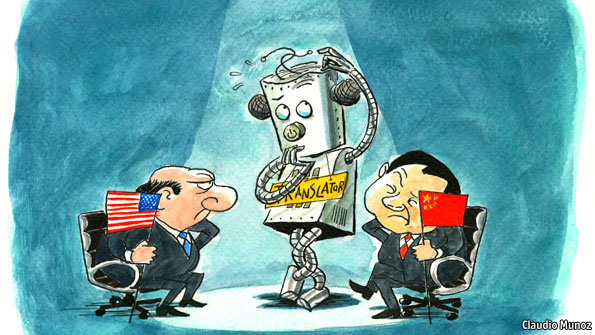
\includegraphics[width=0.5\linewidth]{simtrans/computer-interpreter} \\
      \cite{Hu:Zhai:Eidelman:Boyd-Graber-2014,II:He:Boyd-Graber:Morgan-2014}
       \end{center}
    \vspace{-.4cm}
    \end{block}

  \column{.5\linewidth}



    \begin{block}{Assistive Technology}
     \centering
        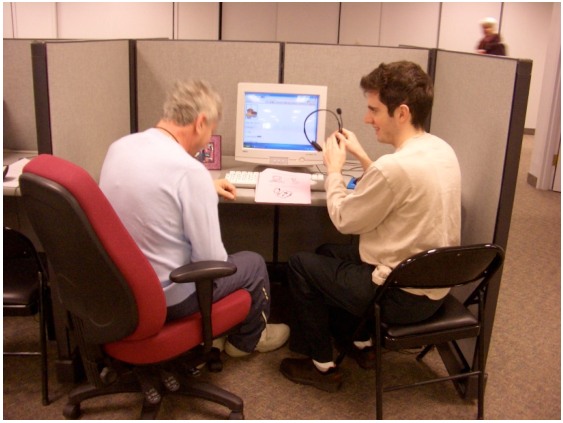
\includegraphics[width=0.4\linewidth]{evocation/figures/jordan_at_adler}
        \\
     \small
       \cite{boyd-graber-06b,ma-09,nikolova-09}
    \end{block}




   \begin{block}{Computational Biology}
     \centering
     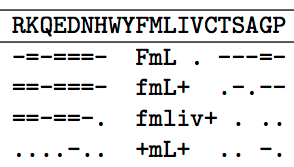
\includegraphics[width=0.4\linewidth]{general_figures/protein} \\
     \small
     \cite{nguyen-13b,hu-13:coalescent}
   \end{block}


\end{columns}

}





\frame{

	\frametitle{Thanks}

        \begin{block}{Collaborators}
          Yuening Hu (UMD), Ke Zhai (UMD), Viet-An Nguyen (UMD), Dave Blei
          (Princeton), Jonathan Chang (Facebook), Philip Resnik (UMD), Christiane Fellbaum (Princeton), Jerry
          Zhu (Wisconsin), Sean Gerrish (Sift), Chong Wang (CMU), Dan Osherson
          (Princeton), Sinead Williamson (CMU)
        \end{block}

        \begin{block}{Funders}
        \end{block}
        \begin{center}
          
\includegraphics[width=0.2\linewidth]{general_figures/nsf}
          \hspace{0.5cm}
          
\includegraphics[width=0.2\linewidth]{general_figures/arl}
          \hspace{0.5cm}
          
\includegraphics[width=0.2\linewidth]{general_figures/iarpa}
          \hspace{0.5cm}
          
\includegraphics[width=0.2\linewidth]{general_figures/lockheed-martin}
       \end{center}

}




\begin{frame}{References}
\bibliographystyle{style/acl}
\tiny
\bibliography{bib/journal-full,bib/jbg,bib/vietan}
\end{frame}



\begin{frame}{Latent Dirichlet Allocation: A Generative Model}

\begin{itemize}
\item Focus in this talk: statistical methods
  \begin{itemize}
    \item Model: story of how your data came to be
    \item Latent variables: missing pieces of your story
    \item Statistical inference: filling in those missing pieces
  \end{itemize}
\item We use latent Dirichlet allocation (LDA)~\cite{blei-03}, a fully Bayesian
  version of pLSI~\cite{hofmann-99}, probabilistic version of
  LSA~\cite{landauer-97}
\end{itemize}

\end{frame}

\frame
{
  \frametitle{Latent Dirichlet Allocation: A Generative Model}

\begin{center}
\only<1>{ 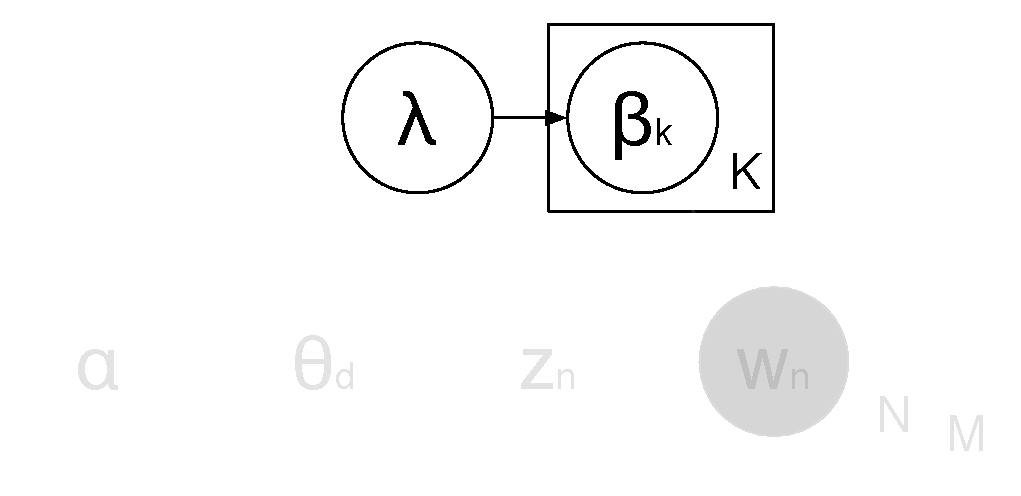
\includegraphics[scale=0.4]{topic_models/lda1.pdf} }
\only<2>{ 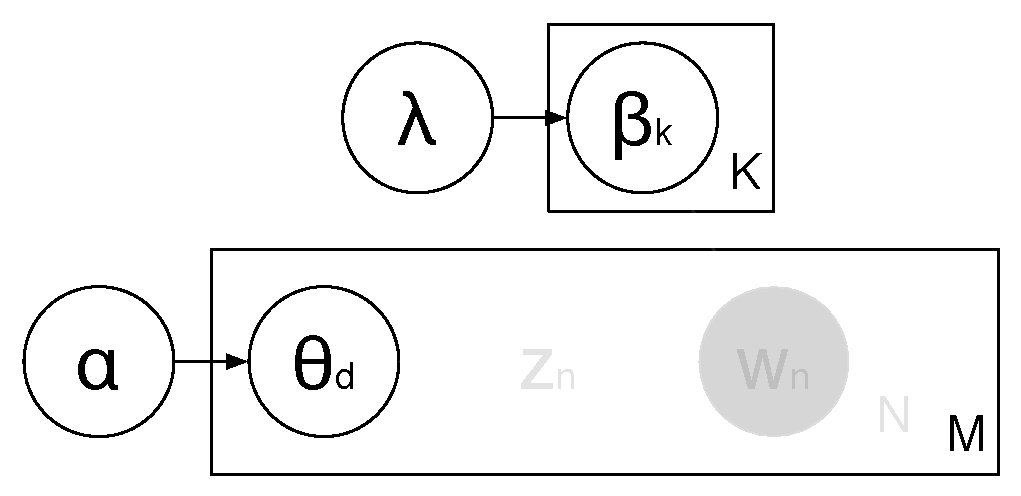
\includegraphics[scale=0.4]{topic_models/lda2.pdf} }
\only<3>{ 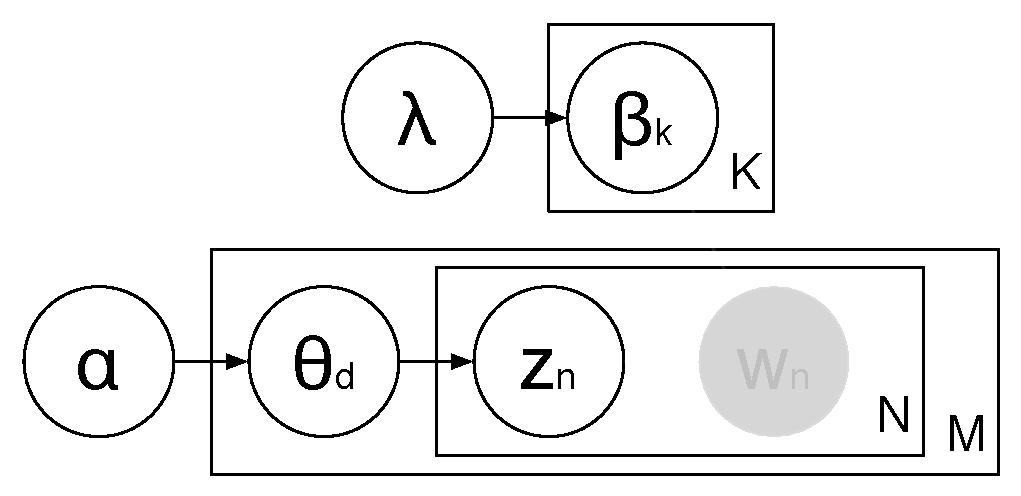
\includegraphics[scale=0.4]{topic_models/lda3.pdf} }
\only<4->{ 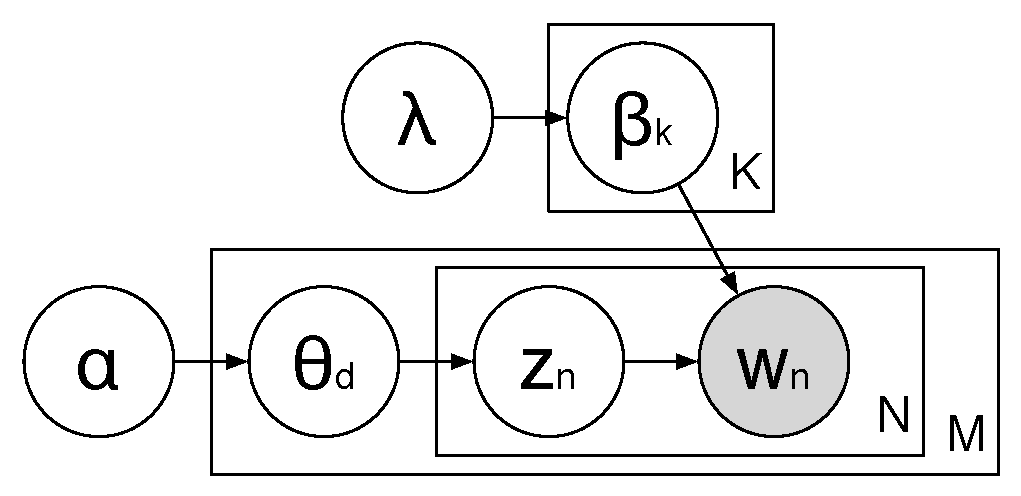
\includegraphics[scale=0.4]{topic_models/lda4.pdf} }
\end{center}

\begin{itemize}
\item<1-> For each topic $k \in \{1, \dots, K\}$, draw a multinomial distribution $\beta_k$ from a Dirichlet distribution with parameter $\lambda$
\item<2-> For each document $d \in \{1, \dots, M\}$, draw a multinomial distribution $\theta_d$ from a Dirichlet distribution with parameter $\alpha$
\item<3-> For each word position $n \in \{1, \dots, N\}$, select a hidden topic $z_n$ from the multinomial distribution parameterized by $\theta$.
\item<4-> Choose the observed word $w_n$ from the distribution $\beta_{z_n}$.
\end{itemize}

\only<5->{We use statistical inference to uncover the most likely unobserved variables given observed data.}
}

\begin{frame}

	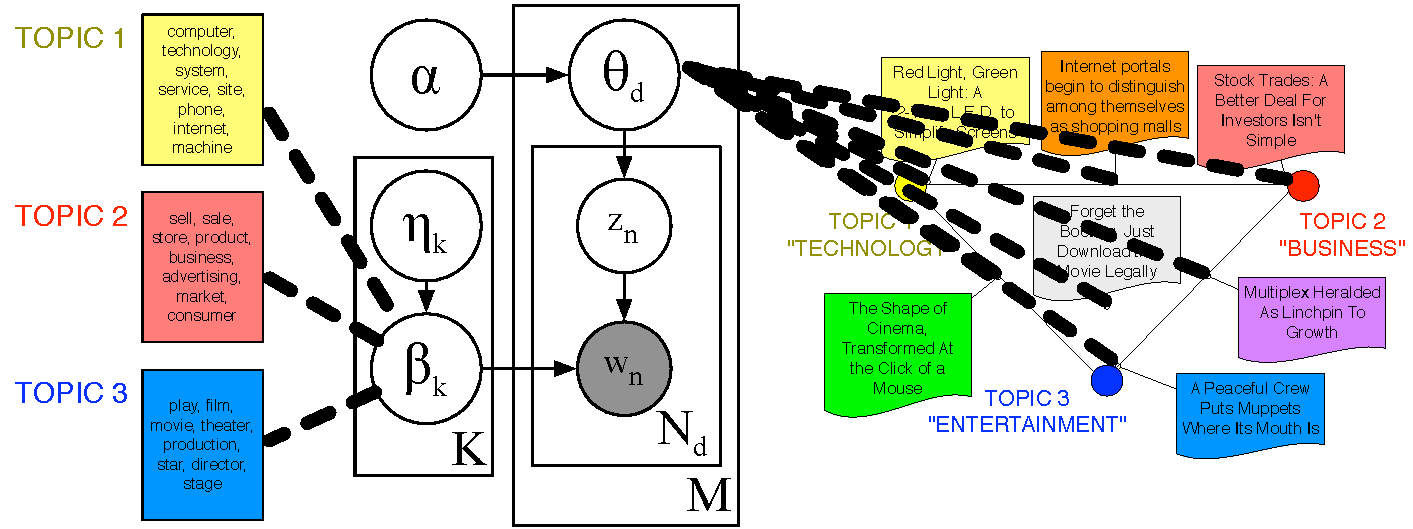
\includegraphics[width=1.0\linewidth]{mrlda/lda_graphmod_nyt}

\end{frame}


\begin{frame}{SHLDA Model}
                    \centering
    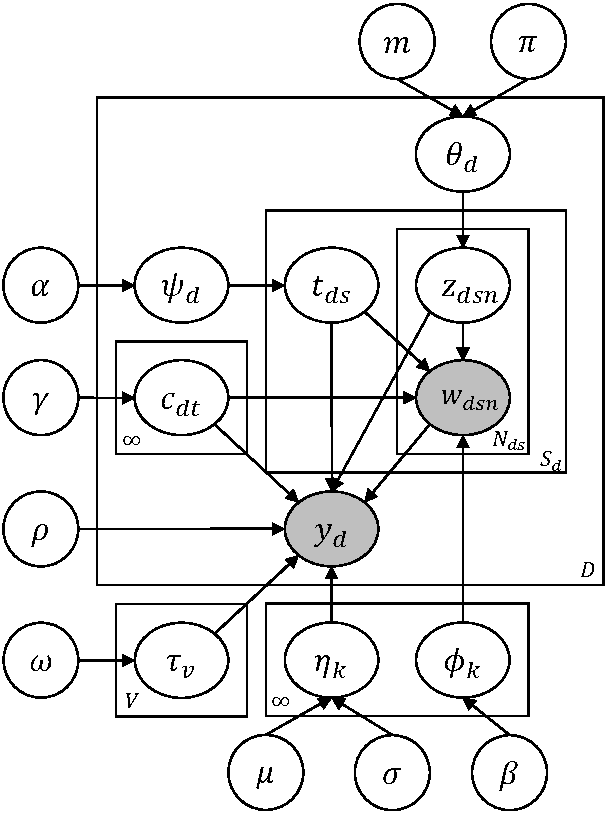
\includegraphics[width=.5\linewidth]{shlda/shLDA}
\end{frame}


\begin{frame}
\frametitle{Infvoc Classification Accuracy}

\begin{table}[tb]
\centering
%\begin{footnotesize}
\begin{tabular}{ c | c | c | c | c}
%\hline
%\multicolumn{4}{c|}{model settings} & accuracy $\%$ \\
\hline
\multirow{10}{*}{ \begin{sideways}{\visible<1->{$S=155$}}\end{sideways}} &
\multirow{9}{*}{\begin{sideways}{\visible<1->{$\tau_0=64$
      $\kappa=0.6$}}\end{sideways}} & \visible<3->{\textit{infvoc}} &
\visible<3->{$\alpha^\beta=3k$ $T=40k$ $U=10$} & \visible<3->{$52.683$} \\
\cline{3-5}
& & \visible<1->{\textit{fixvoc}} & \visible<1->{vb-dict} & \visible<1->{$45.514$} \\
& & \visible<4->{\textit{fixvoc}} & \visible<4->{vb-null} & \visible<4->{$49.390$} \\
& & \visible<4->{\textit{fixvoc}} & \visible<4->{hybrid-dict} & \visible<4->{$46.720$} \\
& & \visible<4->{\textit{fixvoc}} & \visible<4->{hybrid-null} & \visible<4->{$50.474$} \\
\cline{3-5}
& & \visible<2->{\textit{fixvoc-hash}} & \visible<2->{vb-dict} & \visible<2->{$52.525$} \\
& & \visible<4->{\textit{fixvoc-hash}} & \visible<4->{vb-full $T=30k$} & \visible<4->{$51.653$} \\
& & \visible<4->{\textit{fixvoc-hash}} & \visible<4->{hybrid-dict} & \visible<4->{$50.948$} \\
& & \visible<4->{\textit{fixvoc-hash}} & \visible<4->{hybrid-full $T=30k$} & \visible<4->{$50.948$} \\
\cline{2-5}
& \multicolumn{3}{c|}{\visible<5->{\textit{dtm-dict} $tcv=0.001$}} & \visible<5->{$62.845$} \\
\hline
\end{tabular}
%\end{footnotesize}
\caption{Classification accuracy based on $50$ topic features
  extracted from \textit{20 newsgroups} data.}
% \label{tbl:20-news-class}
\end{table}

\only<2->{
\begin{center}
Topics learned with \textit{hashing} are no longer interpretable, they
can only be used as features.
\end{center}}

\end{frame}


\providecommand{\dirfunc}[3]{ \frac{ \prod_{#1}^{#2} \g{ #3 } } { \g{ \sum_{#1}^{#2} #3 }}}
\providecommand{\dirnum}[4]{ \frac{\g{ #3 }}{#4} \prod_{#1}^{#2} }
\providecommand{\dirden}[3]{ \g{ \sum_{#1}^{#2} #3 } }

\begin{frame}
\frametitle{Inference}

\begin{itemize}
\item We are interested in posterior distribution
\begin{equation}
p(Z | X, \Theta)
\end{equation}
\pause
\item Here, latent variables are topic assignments $z$ and topics $\theta$.  $X$ is the words (divided into documents), and $\Theta$ are hyperparameters to Dirichlet distributions: $\alpha$ for topic proportion, $\lambda$ for topics.
\begin{equation}
p({\bm z}, {\bm \beta}, {\bm \theta} | {\bm w}, \alpha, \lambda)
\end{equation}
\pause
\begin{align*}
p({\bm w}, {\bm z}, {\bm \theta}, {\bm \beta} & | \alpha, \lambda) = \\
& \prod_{k} p(\beta_k | \lambda) \prod_{d} p(\theta_d | \alpha) \prod_{n}
p(z_{d,n} | \theta_d) p(w_{d,n} | \beta_{z_{d,n}})
\end{align*}
\end{itemize}
\end{frame}



\begin{frame}
\frametitle{Gibbs Sampling}
\begin{itemize}
\item A form of Markov Chain Monte Carlo
\item Chain is a sequence of random variable states
\item Given a state $\{z_1, \dots z_N\}$ given certain technical conditions, drawing $z_k \sim p(z_1, \dots z_{k-1}, z_{k+1}, \dots z_N | X, \Theta)$ for all $k$ (repeatedly) results in a Markov Chain whose stationary distribution \emph{is} the posterior.
\item For notational convenience, call ${\bm z}$ with $z_{d,n}$ removed ${\bm z}_{-d,n}$
\end{itemize}
\end{frame}

\frame{
	\frametitle{Inference}
	\begin{center}
\only<1> {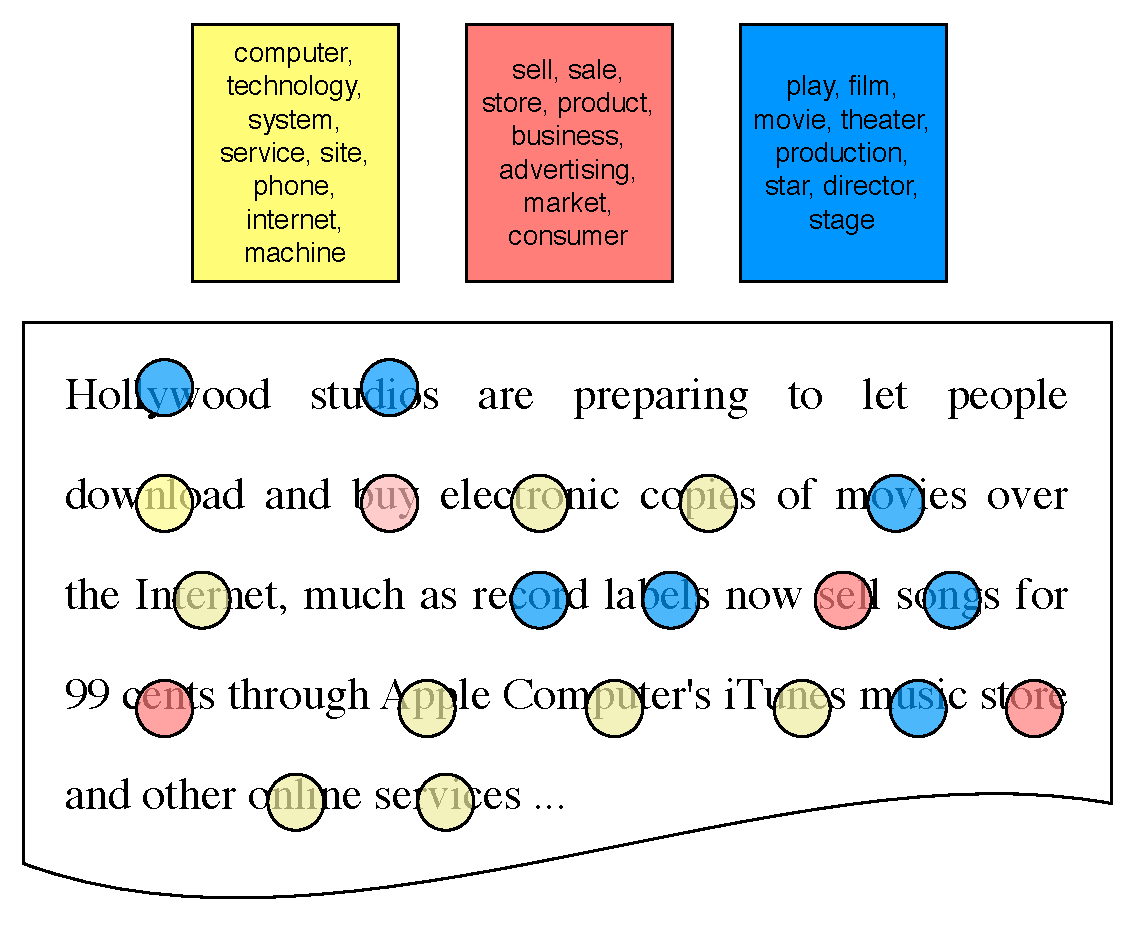
\includegraphics[width=.8\linewidth]{topic_models/inference_3}}
\only<2> {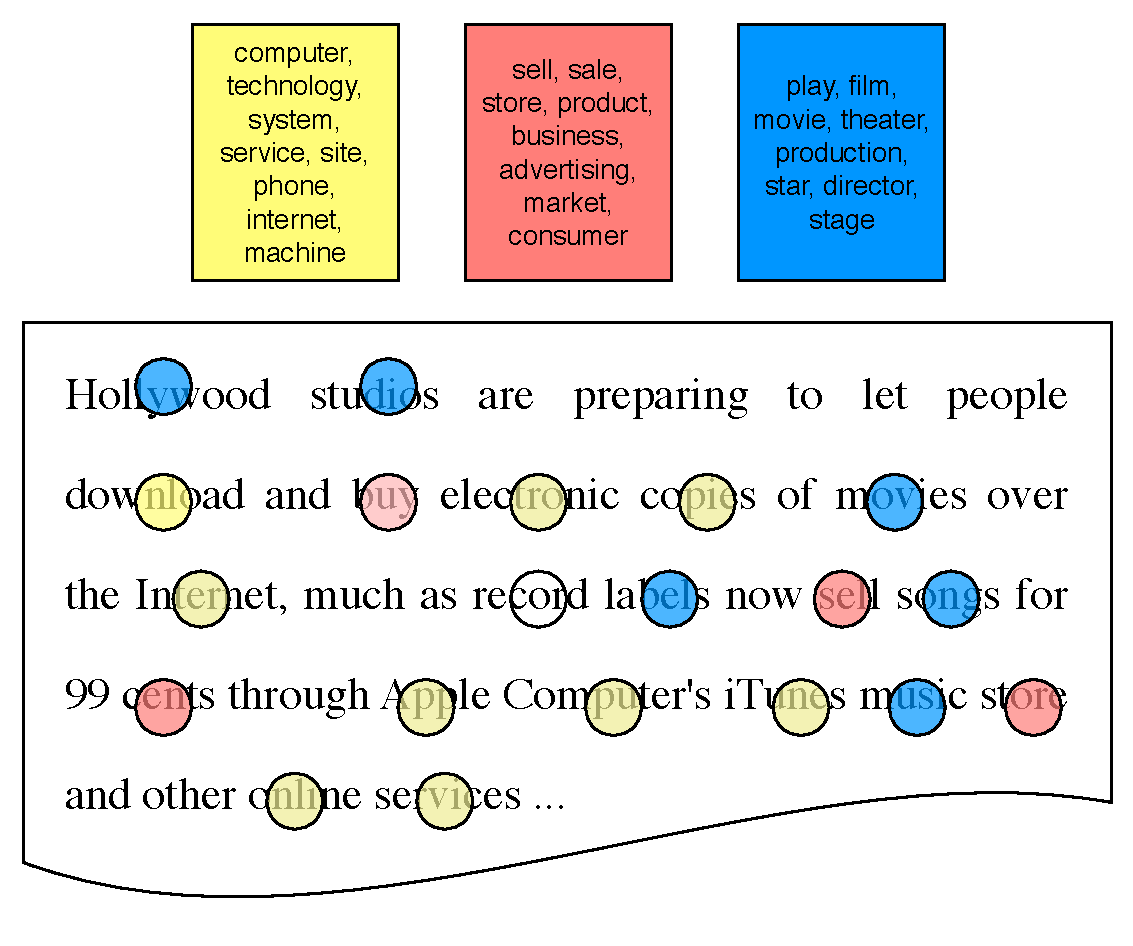
\includegraphics[width=.8\linewidth]{topic_models/inference_4}}
\only<3> {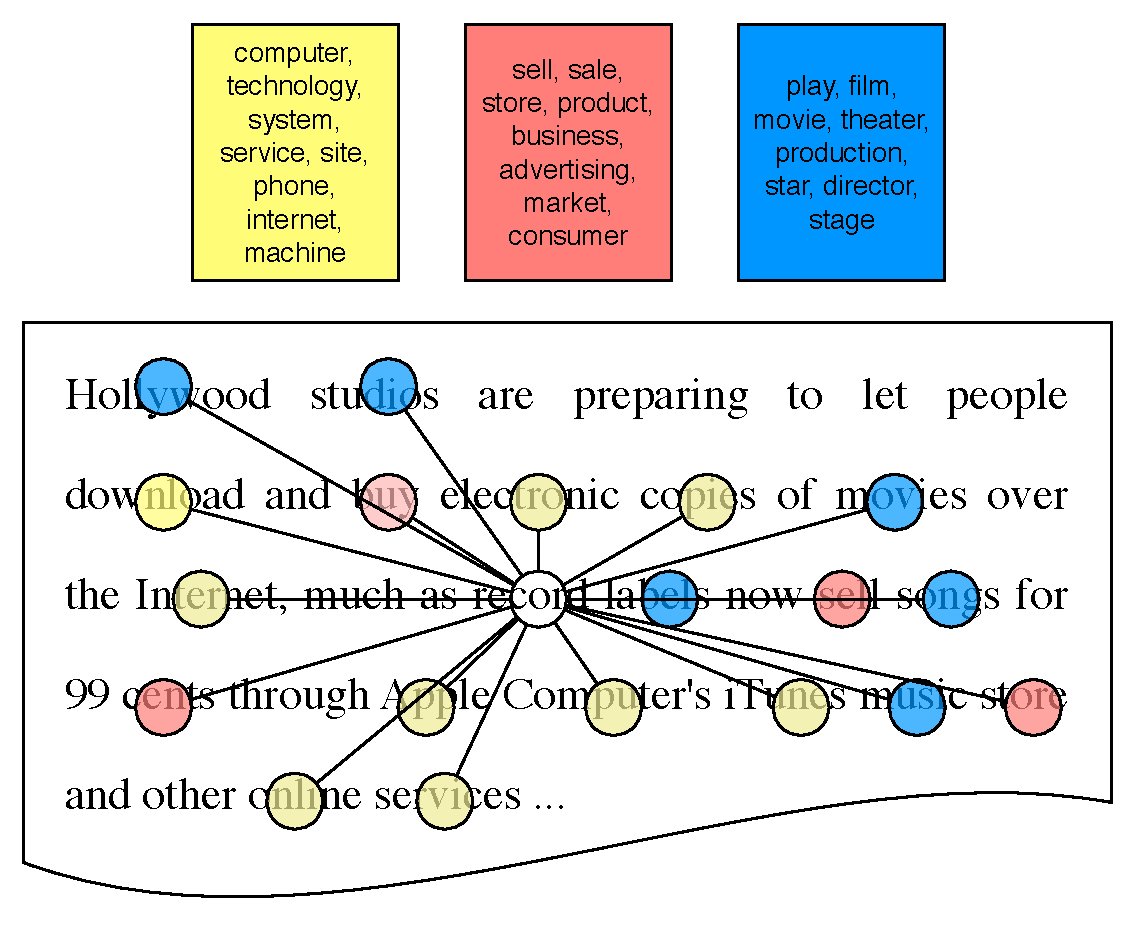
\includegraphics[width=.8\linewidth]{topic_models/inference_5}}
\only<4> {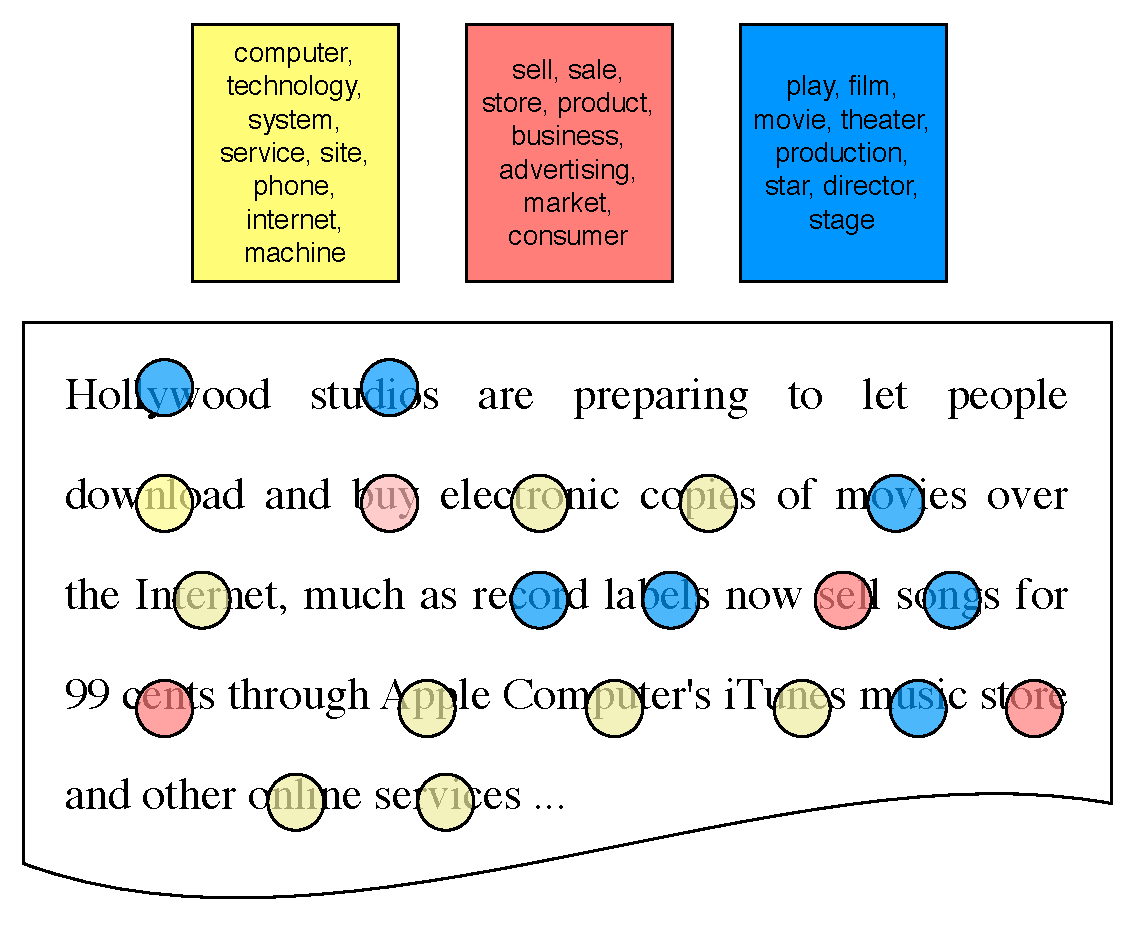
\includegraphics[width=.8\linewidth]{topic_models/inference_3}}
\only<5> {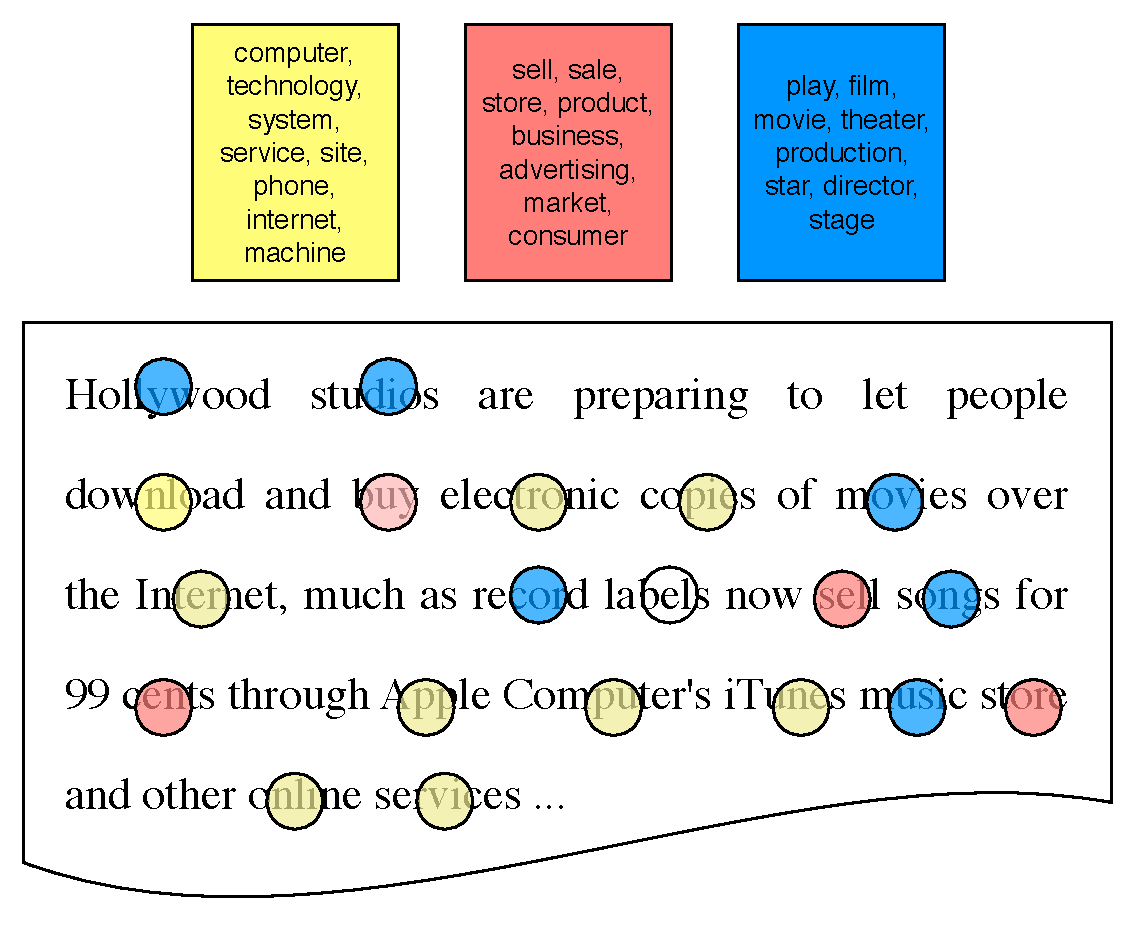
\includegraphics[width=.8\linewidth]{topic_models/inference_6}}
\only<6> {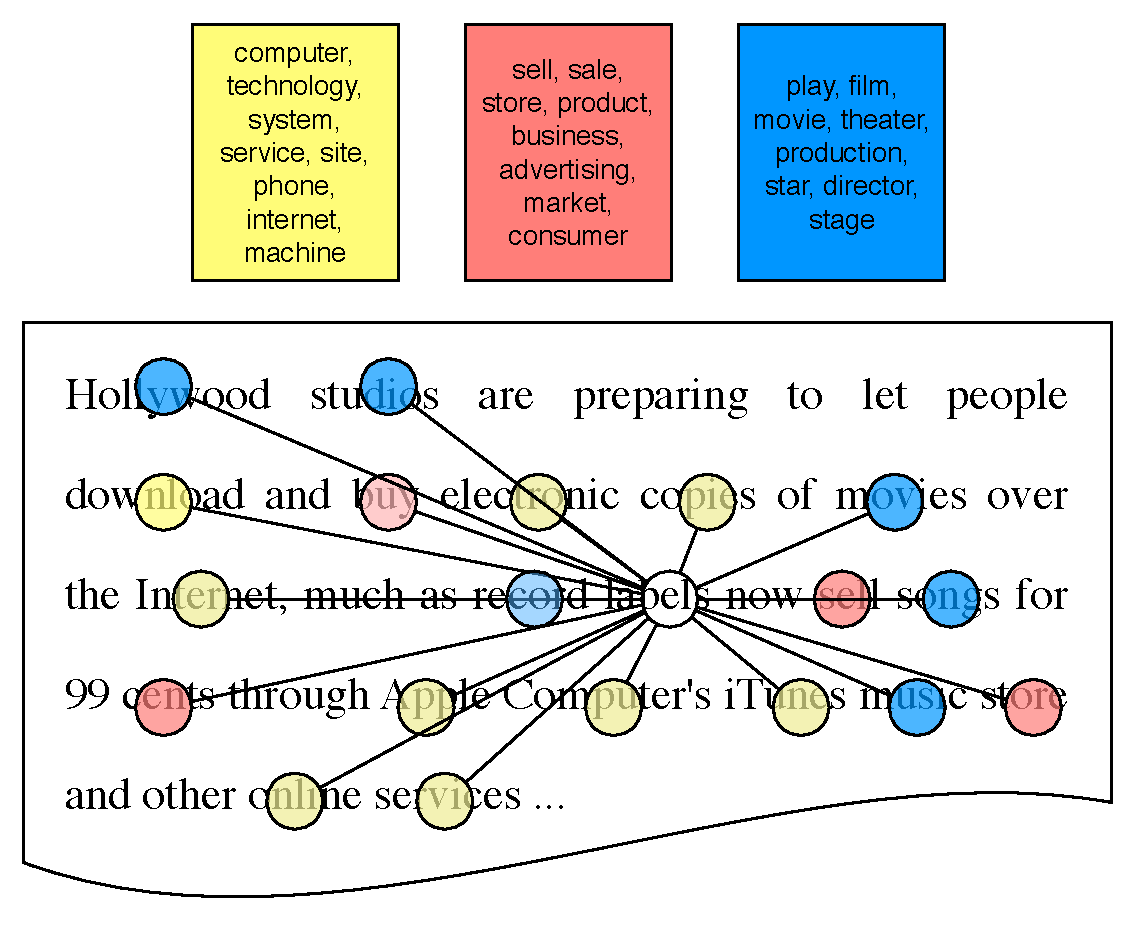
\includegraphics[width=.8\linewidth]{topic_models/inference_7}}
\only<7> {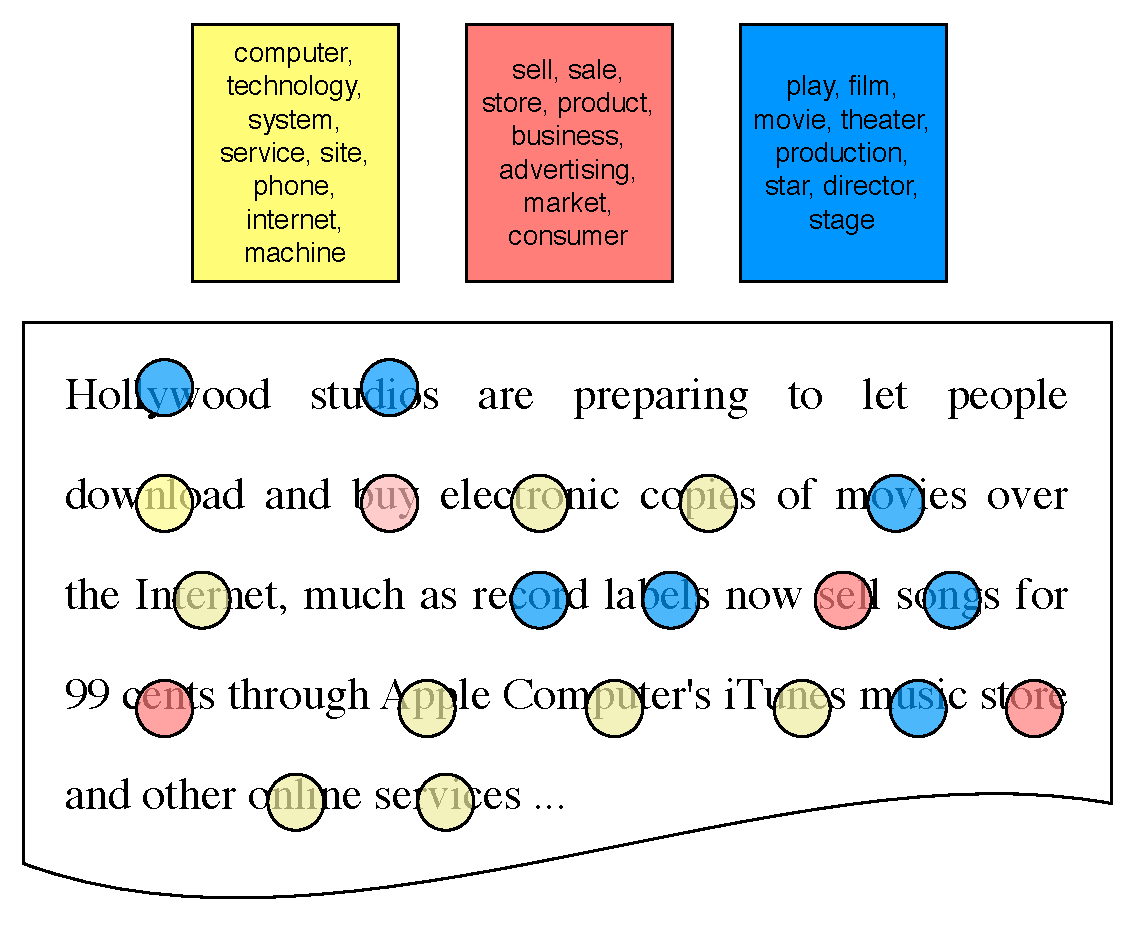
\includegraphics[width=.8\linewidth]{topic_models/inference_3}}
	\end{center}
}


\ifconjugacy

\begin{frame}
\frametitle{Gibbs Sampling}
\begin{itemize}
\item For LDA, we will sample the topic assignments
\item Thus, we want:
\begin{equation*}
p(z_{d,n} = k | {\bm z}_{-d,n}, {\bm w}, \alpha, \lambda) = \frac{ p(z_{d,n} = k, {\bm z}_{-d,n} | {\bm w}, \alpha, \lambda)} { p({\bm z}_{-d,n} | {\bm w},\alpha, \lambda)}
\end{equation*}
\pause
\item The topics and per-document topic proportions are integrated out / marginalized
\item Let $n_{d,i}$ be the number of words taking topic $i$ in document $d$.  Let $v_{k,w}$ be the number of times word $w$ is used in topic $k$.
\end{itemize}


\begin{equation*}
= \frac{ \int_{\theta_d} \left( \prod_{i \not = k} \theta_d^{\alpha_i + n_{d,i} - 1} \right)\theta_d^{\alpha_k + n_{d,i} } d\theta_d \int_{\beta_{k}}    \left( \prod_{i \not = w_{d,n}} \beta_{k,i} ^{ \lambda_i + v_{k,i} - 1} \right) \beta_{k, w_{d,n}}^{\lambda_i + v_{k,i}} d\beta_k } { \int_{\theta_d} \left( \prod_{i} \theta_d^{\alpha_i + n_{d,i} - 1} \right) d\theta_d \int_{\beta_{k}}    \left( \prod_{i} \beta_{k,i} ^{ \lambda_i + v_{k,i} - 1} \right) d\beta_k }
\end{equation*}
\end{frame}

\else

\begin{frame}
\frametitle{Gibbs Sampling}
\begin{itemize}
\item For LDA, we will sample the topic assignments
\item The topics and per-document topic proportions are integrated out / marginalized / Rao-Blackwellized
\item Thus, we want:
\begin{equation*}
p(z_{d,n} = k | {\bm z}_{-d,n}, {\bm w}, \alpha, \lambda) = \frac{n_{d, k} + \alpha_k}{ \sum_{i}^{K} { n_{d,i} + \alpha_i}} \frac{v_{k, w_{d,n}} + \lambda_{w_{d,n}}}{ \sum_{i} { v_{k,i} + \lambda_{i} }}
\end{equation*}
\end{itemize}
\end{frame}

\fi



\ifconjugacy

\begin{frame}
\frametitle{Gibbs Sampling}
\begin{itemize}
\item Integral is normalizer of Dirichlet distribution
\begin{equation*}
\int_{\beta_{k}}    \left( \prod_{i} \beta_{k,i} ^{ \lambda_i + v_{k,i} - 1} \right) d\beta_k = \dirfunc{i}{V}{\beta_i + v_{k,i}}
\end{equation*}
\pause
\item So we can simplify
\end{itemize}
\begin{footnotesize}
\begin{align*}
& \frac{ \int_{\theta_d} \left( \prod_{i \not = k} \theta_d^{\alpha_i + n_{d,i}
      - 1} \right)\theta_d^{\alpha_k + n_{d,i} } d\theta_d \int_{\beta_{k}}
  \left( \prod_{i \not = w_{d,n}} \beta_{k,i} ^{ \lambda_i + v_{k,i} - 1}
  \right) \beta_{k, w_{d,n}}^{\lambda_i + v_{k,i}} d\beta_k } { \int_{\theta_d}
  \left( \prod_{i} \theta_d^{\alpha_i + n_{d,i} - 1} \right) d\theta_d
  \int_{\beta_{k}}    \left( \prod_{i} \beta_{k,i} ^{ \lambda_i + v_{k,i} - 1}
  \right) d\beta_k } = \\
& \frac{
  \dirnum{i \not = k}{K}{\alpha_k + n_{d,k} + 1}{ \g{\sum_{i}^{K} \alpha_i +
      n_{d,i} + 1} } \g{\alpha_k + n_{d,k}}  }
{ \dirfunc{i}{K}{\alpha_i + n_{d,i}} }
% -----------------------------------
\frac{
 \dirnum{i \not = w_{d,n}}{V}{\lambda_{w_{d,n}} + v_{k,w_{d,n}} + 1}{ \g{\sum_{i}^{V} \lambda_i + v_{k,i} + 1} } \g{\lambda_k + v_{k,w_{d,n}}}
}{ \dirfunc{i}{V}{\lambda_i + v_{k,i}} } \\
% -----------------------------------
\end{align*}
\end{footnotesize}
\end{frame}


\begin{frame}

\begin{block}{Gamma Function Identity}
	\begin{equation}
		z = \frac{\Gamma(z + 1)}{\Gamma(z)}
	\end{equation}
\end{block}

\begin{footnotesize}
\begin{align*}
& \frac{
  \dirnum{i \not = k}{K}{\alpha_k + n_{d,k} + 1}{ \g{\sum_{i}^{K} \alpha_i +
      n_{d,i} + 1} } \g{\alpha_k + n_{d,k}}  }
{ \dirfunc{i}{K}{\alpha_i + n_{d,i}} }
% -----------------------------------
\frac{
 \dirnum{i \not = w_{d,n}}{V}{\lambda_{w_{d,n}} + v_{k,w_{d,n}} + 1}{ \g{\sum_{i}^{V} \lambda_i + v_{k,i} + 1} } \g{\lambda_k + v_{k,w_{d,n}}}
}{ \dirfunc{i}{V}{\lambda_i + v_{k,i}} } \\
% -----------------------------------
& = \frac{n_{d, k} + \alpha_k}{ \sum_{i}^{K} { n_{d,i} + \alpha_i}} \frac{v_{k, w_{d,n}} + \lambda_{w_{d,n}}}{ \sum_{i} { v_{k,i} + \lambda_{i} }}
\end{align*}
\end{footnotesize}

\end{frame}
\else
\fi

\begin{frame}{Gibbs Sampling Equation}
  
\begin{equation}
\alert<5>{\frac{\alert<1>{n_{d, k}} +  \alert<3>{\alpha_k}}{ \sum_{i}^{K} { n_{d,i} +\alpha_i}}} \alert<6>{\frac{\alert<2>{v_{k, w_{d,n}}} + \alert<4>{\lambda_{w_{d,n}}}}{ \sum_{i} { v_{k,i} + \lambda_{i} }}}
\end{equation}

\begin{itemize}
  \item \alert<1>{Number of times document $d$ uses topic $k$}
  \item \alert<2>{Number of times topic $k$ uses word type $w_{d,n}$}
  \item \alert<3>{Dirichlet parameter for document to topic
      distribution}
  \item \alert<4>{Dirichlet parameter for topic to word distribution}
  \item \alert<5>{How much this document likes topic $k$}
  \item \alert<6>{How much this topic likes word $w_{d,n}$}
\end{itemize}

\end{frame}

\begin{frame}
  \frametitle{Sample Document}
    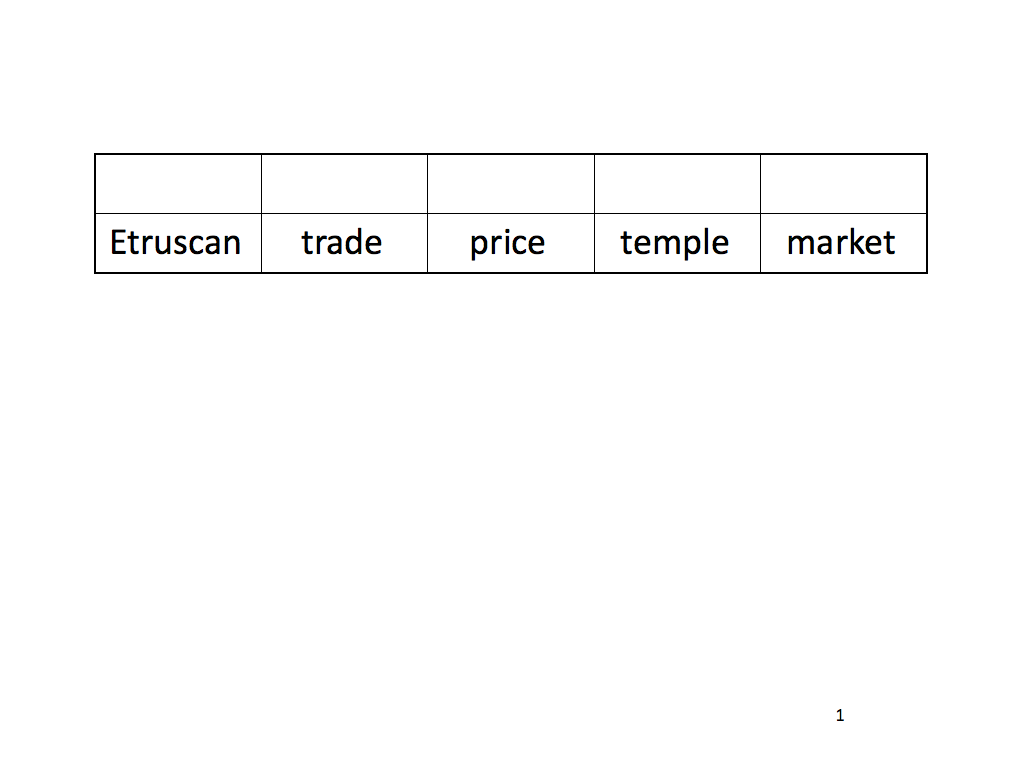
\includegraphics[width=\linewidth]{topic_models/mimno_001}
\end{frame}

\begin{frame}
  \frametitle{Sample Document}
    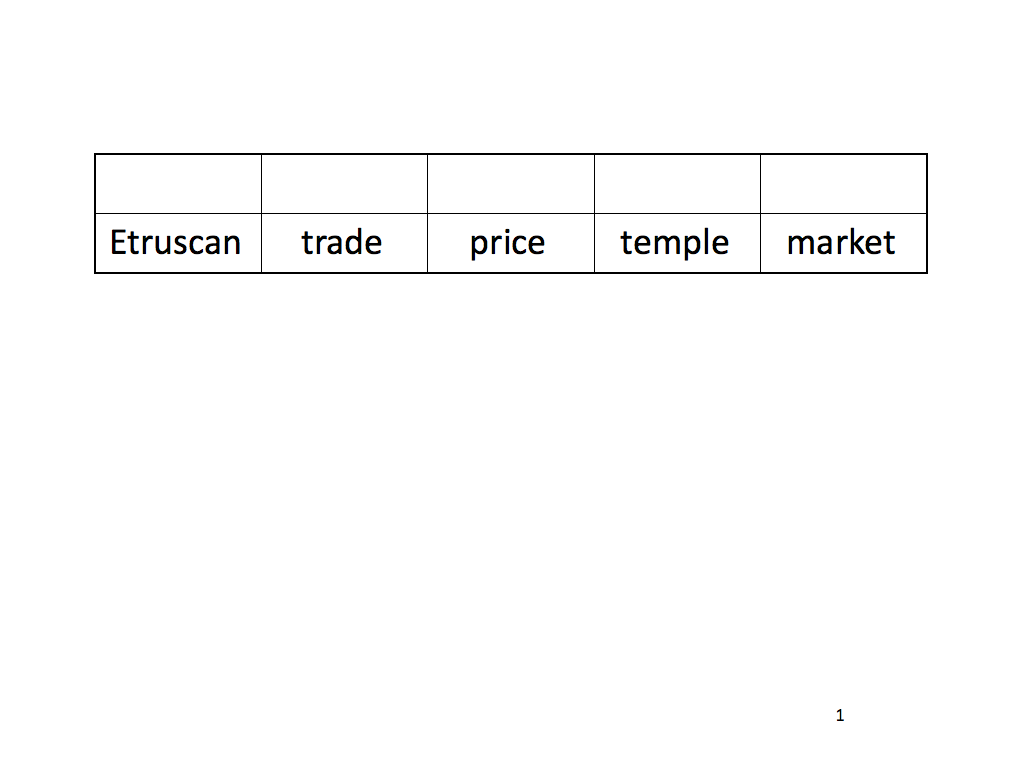
\includegraphics[width=\linewidth]{topic_models/mimno_001}
\end{frame}

\begin{frame}
  \frametitle{Randomly Assign Topics}
    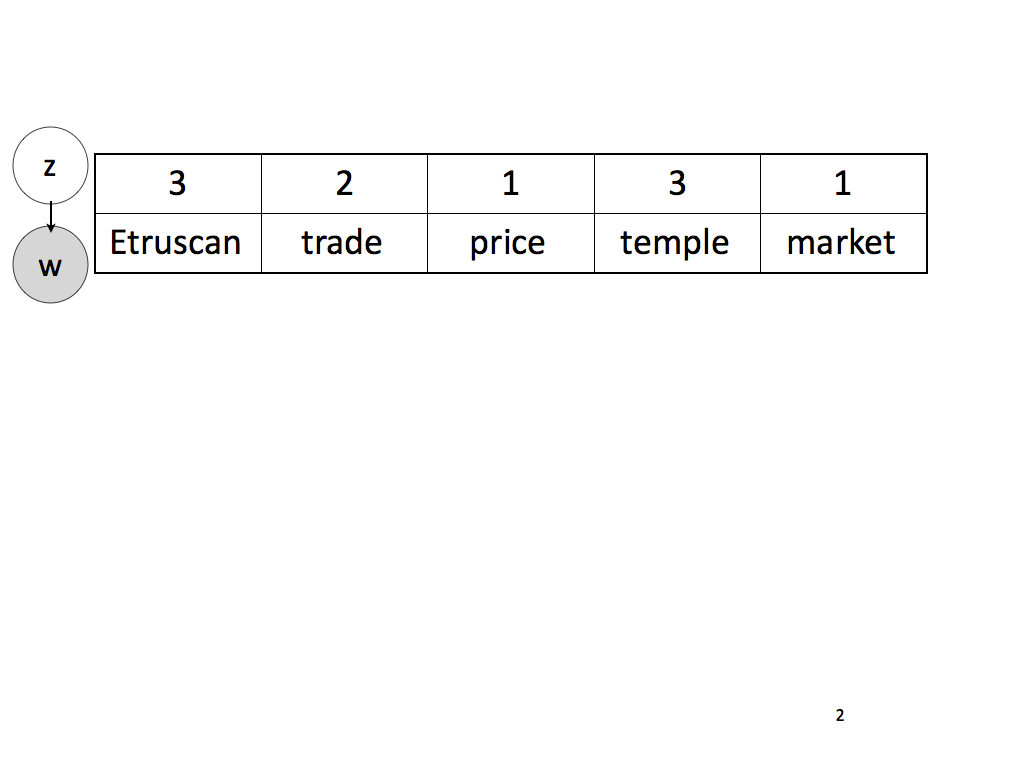
\includegraphics[width=\linewidth]{topic_models/mimno_002}
\end{frame}

\begin{frame}
  \frametitle{Randomly Assign Topics}
    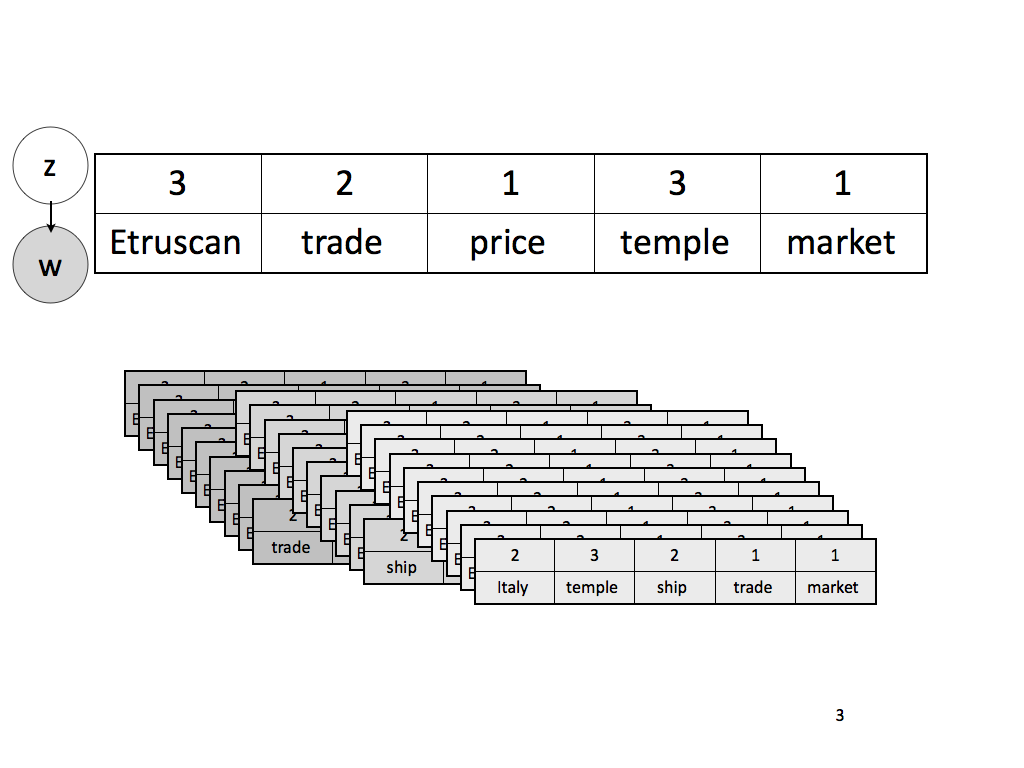
\includegraphics[width=\linewidth]{topic_models/mimno_003}
\end{frame}

\begin{frame}
  \frametitle{Total Topic Counts}
    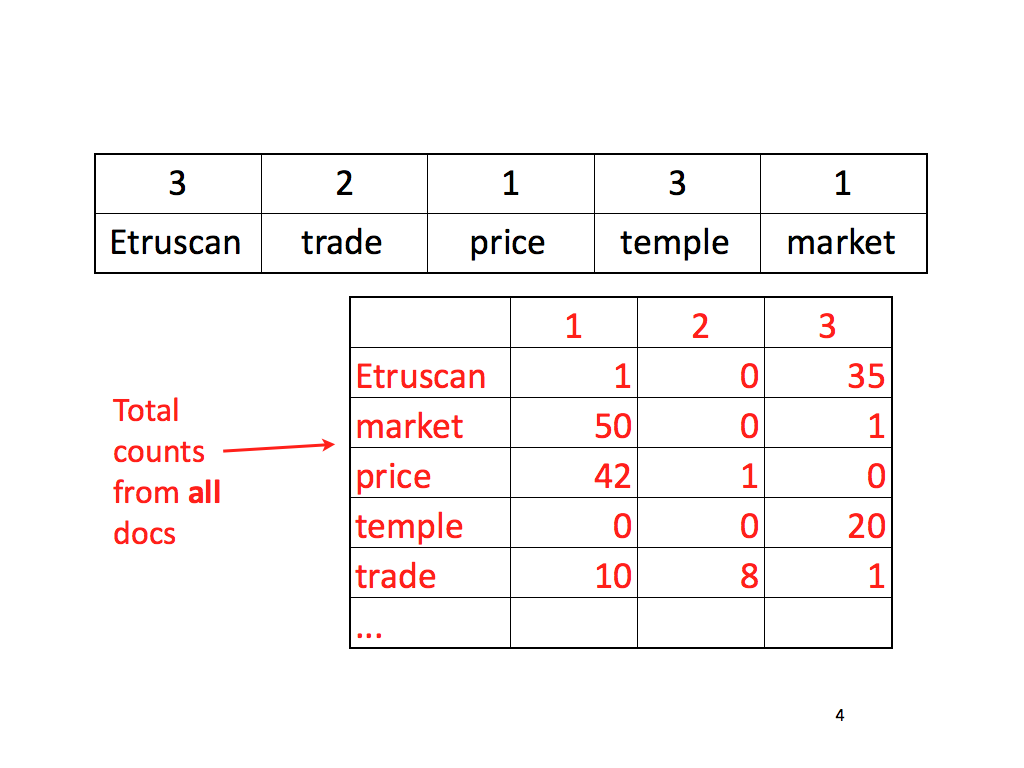
\includegraphics[width=\linewidth]{topic_models/mimno_004}

\pause

\vspace{-3cm}

\begin{block}{Sampling Equation}
	\begin{equation*}
          \frac{n_{d, k} + \alpha_k}{ \sum_{i}^{K} { n_{d,i} + \alpha_i}} \frac{\alert<3>{v_{k, w_{d,n}}} + \lambda_{w_{d,n}}}{ \sum_{i} { \alert<3>{v_{k,i}} + \lambda_{i} }}
	\end{equation*}
\end{block}

\end{frame}


\begin{frame}
  \frametitle{We want to sample this word \dots}
    \only<1>{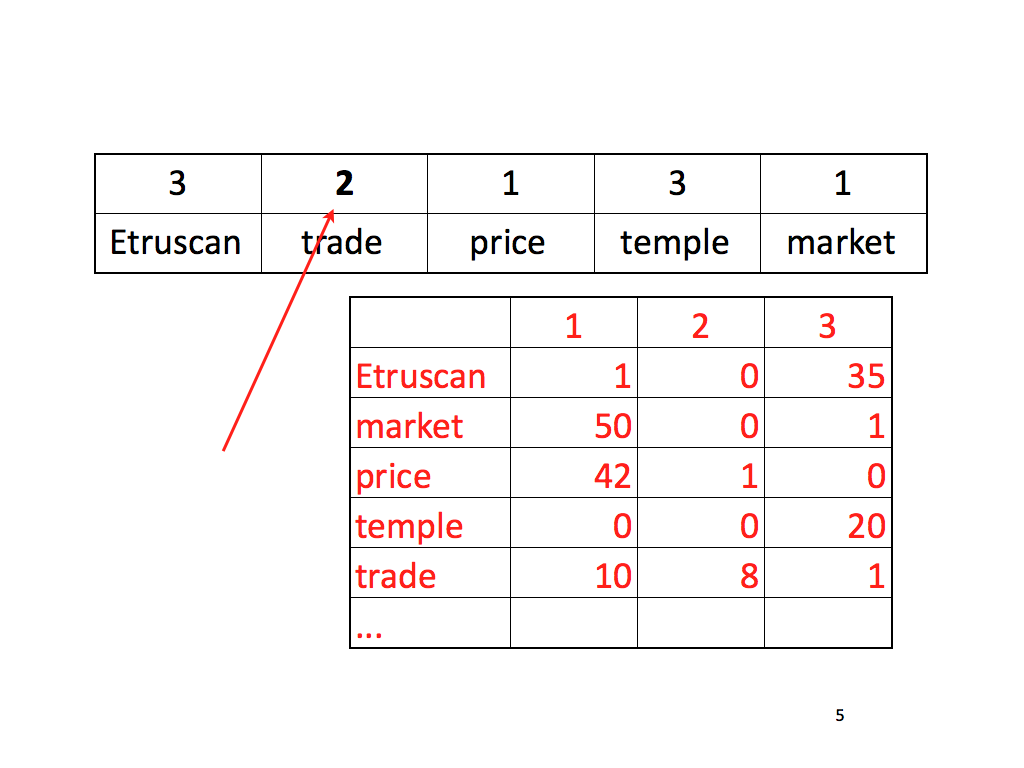
\includegraphics[width=\linewidth]{topic_models/mimno_005}}
    \only<2>{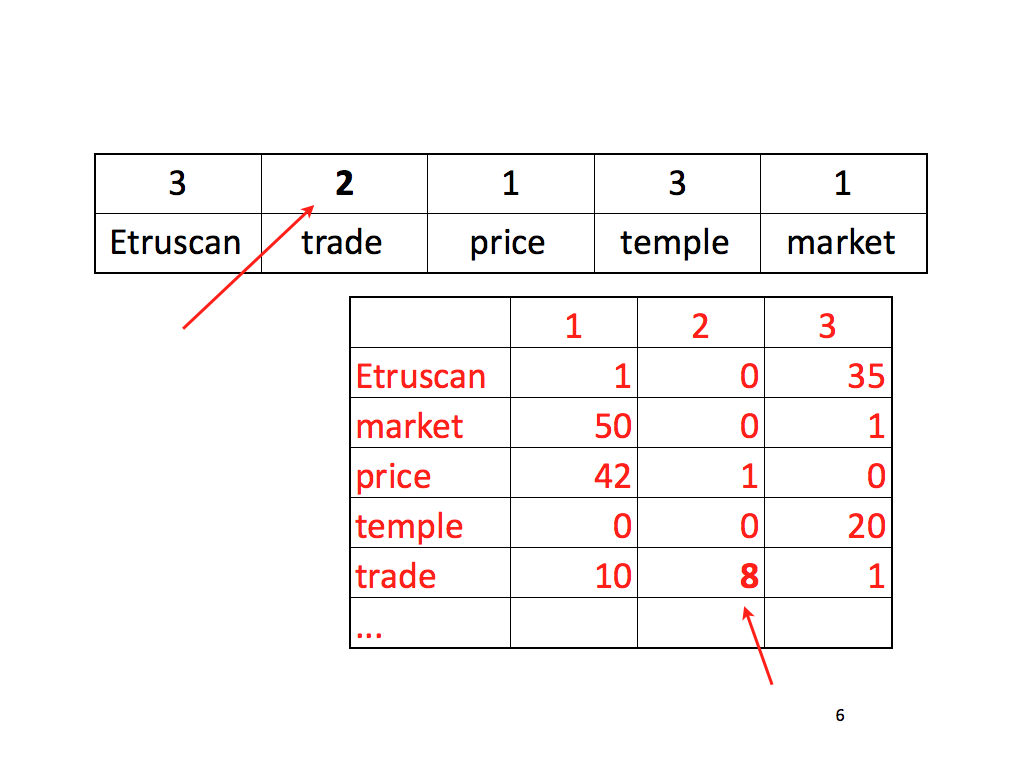
\includegraphics[width=\linewidth]{topic_models/mimno_006}}
\end{frame}

\begin{frame}
  \frametitle{Decrement its count}
    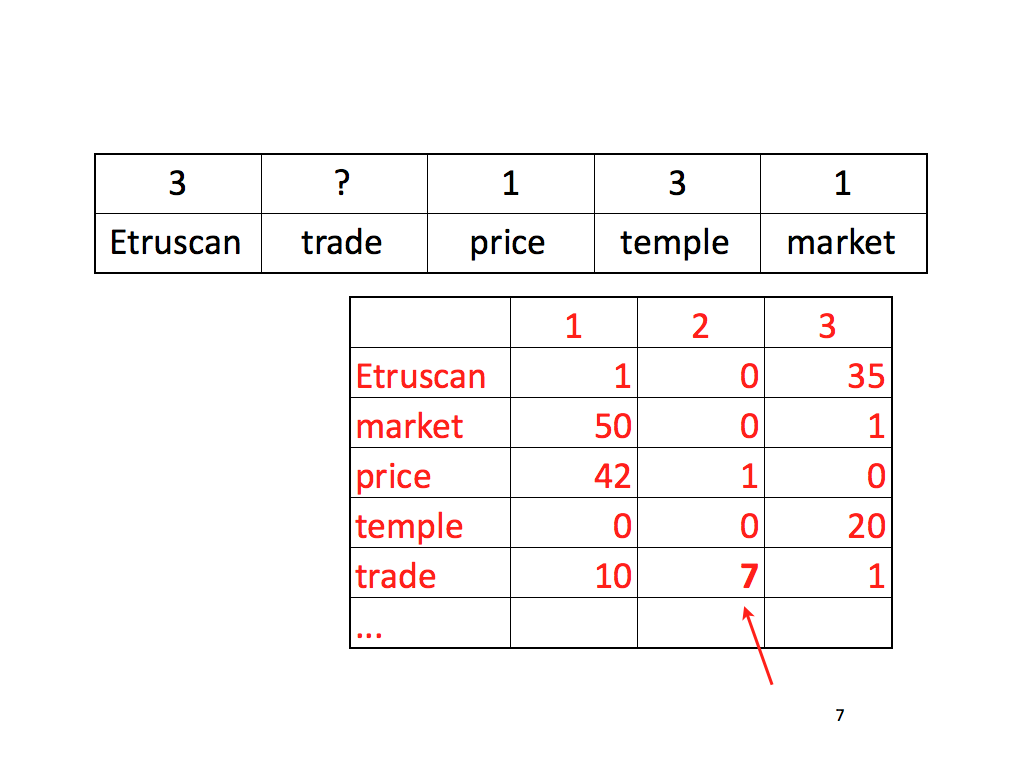
\includegraphics[width=\linewidth]{topic_models/mimno_007}
\end{frame}

\begin{frame}
  \frametitle{What is the conditional distribution for this topic?}
    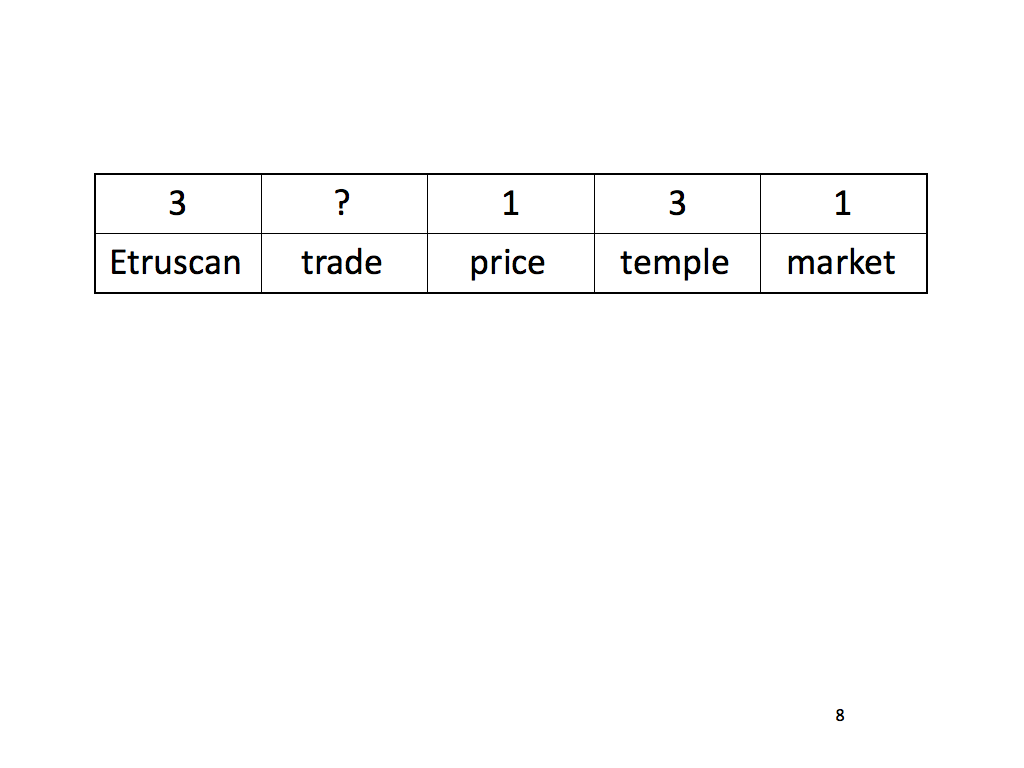
\includegraphics[width=\linewidth]{topic_models/mimno_008}
\end{frame}


\begin{frame}
  \frametitle{Part 1: How much does this document like each topic?}
    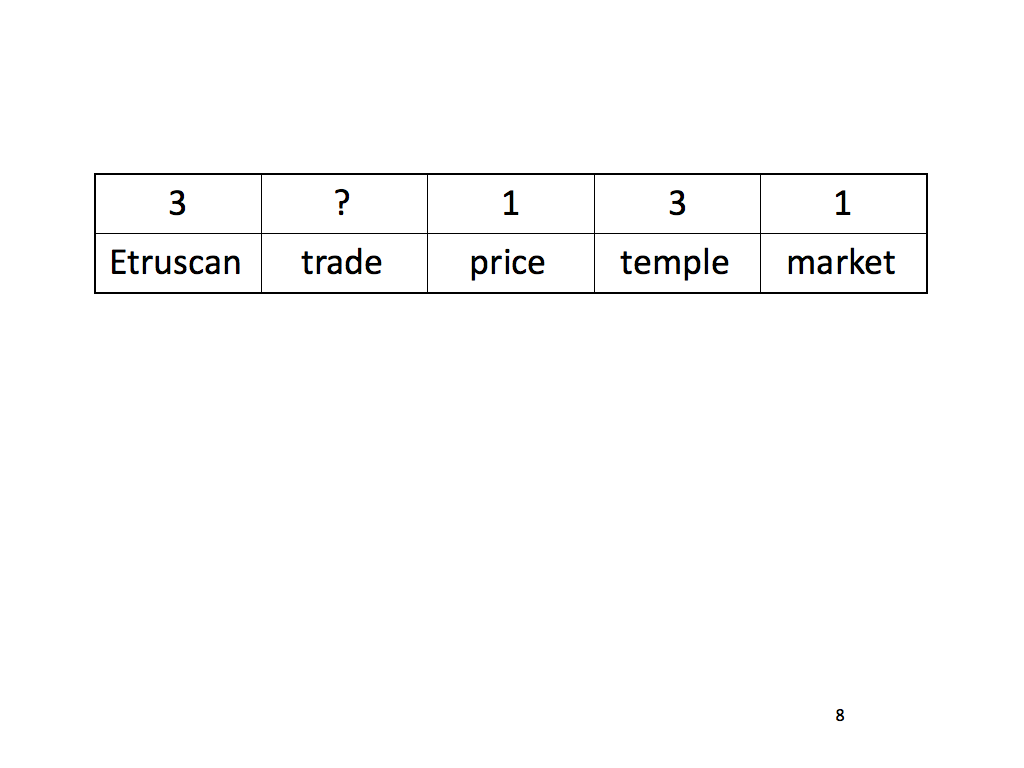
\includegraphics[width=\linewidth]{topic_models/mimno_008}
\end{frame}

\begin{frame}
  \frametitle{Part 1: How much does this document like each topic?}
    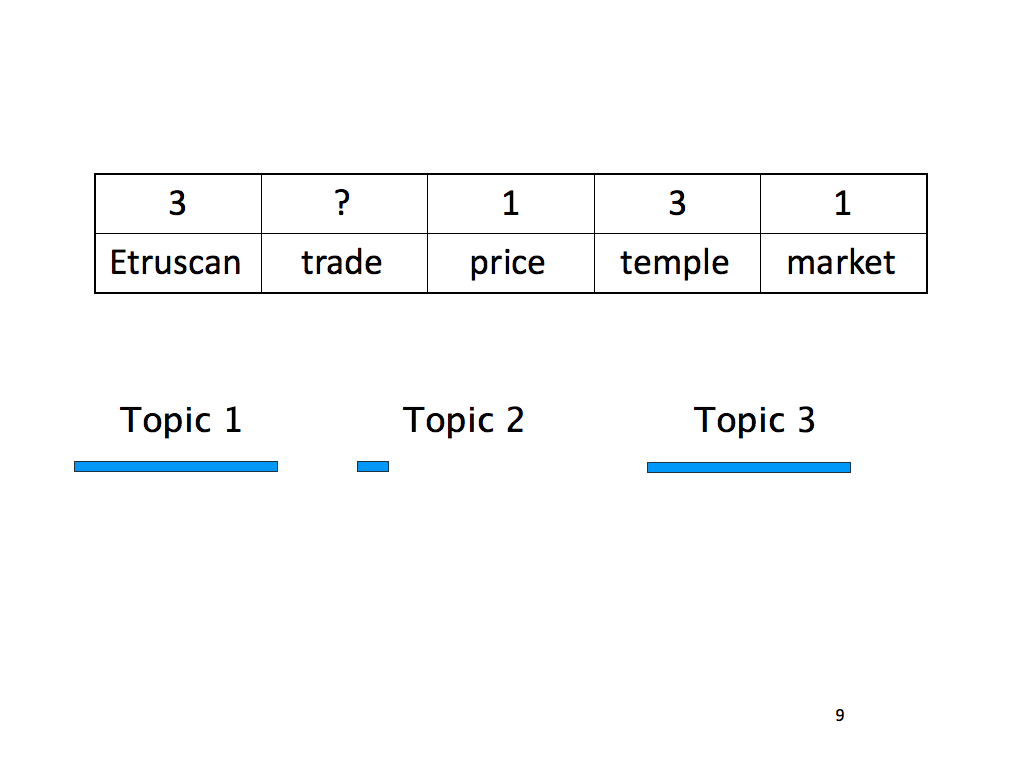
\includegraphics[width=\linewidth]{topic_models/mimno_009}

    \pause
    \vspace{-4cm}
    \begin{block}{Sampling Equation}
	\begin{equation*}
          \frac{\alert<3>{n_{d, k}} + \alpha_k}{ \sum_{i}^{K} { \alert<3>{n_{d,i}} + \alpha_i}} \frac{v_{k, w_{d,n}} + \lambda_{w_{d,n}}}{ \sum_{i} { v_{k,i} + \lambda_{i} }}
	\end{equation*}
     \end{block}


\end{frame}


\begin{frame}
  \frametitle{Part 2: How much does each topic like the word?}
    \includegraphics[width=\linewidth]{topic_models/mimno_010}

\pause

\vspace{-3cm}

\begin{block}{Sampling Equation}
	\begin{equation*}
          \frac{n_{d, k} + \alpha_k}{ \sum_{i}^{K} { n_{d,i} + \alpha_i}} \frac{\alert<3>{v_{k, w_{d,n}}} + \lambda_{w_{d,n}}}{ \sum_{i} { \alert<3>{v_{k,i}} + \lambda_{i} }}
	\end{equation*}
\end{block}

\end{frame}


\begin{frame}
  \frametitle{Geometric interpretation}
    \only<1>{\includegraphics[width=\linewidth]{topic_models/mimno_011}}
    \only<2>{\includegraphics[width=\linewidth]{topic_models/mimno_012}}
    \only<3>{\includegraphics[width=\linewidth]{topic_models/mimno_013}}
\end{frame}

\begin{frame}
  \frametitle{Update counts}
    \only<1>{\includegraphics[width=\linewidth]{topic_models/mimno_014}}
    \only<2>{\includegraphics[width=\linewidth]{topic_models/mimno_015}}
    \only<3>{\includegraphics[width=\linewidth]{topic_models/mimno_016}}
\end{frame}


\begin{frame}
  \frametitle{Details: how to sample from a distribution}

\begin{center}
  \includegraphics[width=.8\linewidth]{topic_models/sampling_from_distribution}
\end{center}
\end{frame}

\begin{frame}

\begin{block}{Algorithm}
\begin{enumerate}
\item For each iteration $i$:
\begin{enumerate}
\item For each document $d$ and word $n$ currently assigned to $z_{old}$:
\begin{enumerate}
\item Decrement $n_{d,z_{old}}$ and $v_{z_{old}, w_{d,n}}$
\item Sample $z_{new} = k$ with probability proportional to $\frac{n_{d, k} + \alpha_k}{ \sum_{i}^{K} { n_{d,i} + \alpha_i}} \frac{v_{k, w_{d,n}} + \lambda_{w_{d,n}}}{ \sum_{i} { v_{k,i} + \lambda_{i}}}$
\item Increment $n_{d,z_{new}}$ and $v_{z_{new}, w_{d,n}}$
\end{enumerate}
\end{enumerate}
\end{enumerate}
\end{block}

\end{frame}

\begin{frame}

\frametitle{Implementation}

\begin{block}{Algorithm}
\begin{enumerate}
\item For each iteration $i$:
\begin{enumerate}
\item For each document $d$ and word $n$ currently assigned to $z_{old}$:
\begin{enumerate}
\item Decrement $n_{d,z_{old}}$ and $v_{z_{old}, w_{d,n}}$
\item Sample $z_{new} = k$ with probability proportional to $\frac{n_{d, k} + \alpha_k}{ \sum_{i}^{K} { n_{d,i} + \alpha_i}} \frac{v_{k, w_{d,n}} + \lambda_{w_{d,n}}}{ \sum_{i} { v_{k,i} + \lambda_{i}}}$
\item Increment $n_{d,z_{new}}$ and $v_{z_{new}, w_{d,n}}$
\end{enumerate}
\end{enumerate}
\end{enumerate}
\end{block}

\end{frame}


\begin{frame}
\frametitle{Desiderata}
\begin{itemize}
\item Hyperparameters: Sample them too (slice sampling)
\item Initialization: Random
\item Sampling: Until likelihood converges
\item Lag / burn-in: Difference of opinion on this
\item Number of chains: Should do more than one
\end{itemize}
\end{frame}

\begin{frame}
	\frametitle{Available implementations}

	\begin{itemize}
		\item Mallet (http://mallet.cs.umass.edu)
		\item LDAC (http://www.cs.princeton.edu/~blei/lda-c)
		\item Topicmod (http://code.google.com/p/topicmod)
	\end{itemize}
\end{frame}


\begin{frame}

\frametitle{Unassign $(d,n,w_{d,n},z_{d,n} = k)$} 
\begin{algorithmic}[1]
\STATE $T:~T_{d,k} \leftarrow T_{d,k}-1$
\STATE If~$w_{d,n}~\notin~\Omega^{old}$,\\
~~$P:~P_{k, w_{d,n}} \leftarrow P_{k, w_{d,n}} - 1$\\
\STATE Else: suppose $w_{d,n} \in \Omega^{old}_m$,\\
~~$P:~P_{k, m} \leftarrow P_{k, m} - 1$\\
~~$W:~W_{k,m,w_{d,n}} \leftarrow W_{k,m,w_{d,n}} - 1$
\end{algorithmic}
	

\end{frame}


\begin{frame}

	\frametitle{SparseLDA}

\begin{align}	
	\label{eq:fast-lda}
p(z &= k | Z_{-}, w) \propto (\alpha_k + n_{k|d})\frac{\beta + n_{w|k}}{\beta V + n_{\cdot |k}} \\
&\propto \explain{$s_{\textsc{LDA}}$}{\frac{\alpha_k \beta}{\beta V + n_{\cdot |k}}} + \explain{$r_{\textsc{LDA}}$}{\frac{n_{k|d} \beta}{\beta V + n_{\cdot |k}}}
+ \explain{$q_{\textsc{LDA}}$}{\frac{(\alpha_k + n_{k|d})n_{w | k}}{\beta V +
    n_{\cdot |k}}} \notag
\end{align}

\end{frame}


\begin{frame}

	\frametitle{Tree-based sampling}
	
	\begin{align}
\label{eq:naive-ldawn}
p(z_{d,n} &= k, l_{d,n} = \lambda | Z_{-}, L_{-}, w_{d,n}) \\
&\propto (\alpha_k + n_{k|d})
\prod_{(i \rightarrow j)\in \lambda} \frac{\beta_{i \rightarrow j} + n_{i \rightarrow j | k}}
{\sum_{j\prime}{(\beta_{i \rightarrow j'} + n_{i \rightarrow j' | k})}}  \notag
\end{align}

\end{frame}


\begin{frame}

	\frametitle{Factorizing Tree-Based Prior}


\begin{align}
\label{eq:fast-lda}
p(z &= k | Z_{-}, w) \propto (\alpha_k + n_{k|d})\frac{\beta + n_{w|k}}{\beta V + n_{\cdot |k}} \\
&\propto \explain{$s_{\textsc{LDA}}$}{\frac{\alpha_k \beta}{\beta V + n_{\cdot |k}}} + \explain{$r_{\textsc{LDA}}$}{\frac{n_{k|d} \beta}{\beta V + n_{\cdot |k}}}
+ \explain{$q_{\textsc{LDA}}$}{\frac{(\alpha_k + n_{k|d})n_{w | k}}{\beta V +
    n_{\cdot |k}}} \notag
\end{align}
\pause

\begin{align}
\label{eq:smoothing}
s &= \sum_{k,\lambda} \frac{\alpha_k \prod_{(i \rightarrow j)\in \lambda}{\beta_{i \rightarrow j}}}{\prod_{(i \rightarrow j)\in \lambda} {\sum_{j\prime}{(\beta_{i \rightarrow j'} + n_{i \rightarrow j' | k})}}} \notag \\
&\le \sum_{k,\lambda} \frac{\alpha_k \prod_{(i \rightarrow j)\in \lambda}{\beta_{i \rightarrow j}}}{\prod_{(i \rightarrow j)\in \lambda} {\sum_{j\prime}{\beta_{i \rightarrow j'}}}} = s'.
\end{align}




\end{frame}

\begin{frame}[fragile]

\begin{small}
\begin{algorithmic}[1]
\FOR{word w in this document}
\STATE sample $=$ rand() $* (s' + r + q)$
\IF{sample $< s'$}
\STATE compute $s$
\STATE sample $=$ sample $* (s+r+q) / (s'+r+q)$
\IF{sample $< s$}
\RETURN topic $k$ and path $\lambda$ sampled from $s$
\ENDIF
\STATE sample $-= s$
\ELSE
\STATE sample $-= s'$
\ENDIF
\IF{sample $< r$}
\RETURN topic $k$ and path $\lambda$ sampled from $r$
\ENDIF
\STATE sample $-= r$
\RETURN topic $k$ and path $\lambda$ sampled from $q$
\ENDFOR
\end{algorithmic}
\end{small}

\end{frame}

\centering
  \begin{tabular}{| c || c | c | c | c |}
\hline
\multicolumn{5}{|c|}{{\bf Number of Topics}}\\
\hline
& T50 & T100 & T200 & T500\\
\hline
\scriptsize{\textsc{Naive}} & $5.700$ & $12.655$ & $29.200$ & $71.223$\\
\scriptsize{\textsc{Fast}} & $4.935$ & $9.222$ & $17.559$ & $40.691$\\
\scriptsize{\textsc{Fast-RB}} & $2.937$ & $4.037$ & $5.880$ & $8.551$\\
\scriptsize{\textsc{Fast-RB-sD}} & $2.675$ & $3.795$ & $5.400$ & $8.363$\\
\scriptsize{\textsc{Fast-RB-sW}} & $2.449$ & $3.363$ & $4.894$ & $7.404$\\
\scriptsize{\textsc{Fast-RB-sDW}} & $2.225$ & $3.241$ & $4.672$ & $7.424$\\
\hline
\multicolumn{5}{|c|}{{\bf Number of Correlations}}\\
\hline
& C50 & C100 & C200 & C500\\
\hline
\scriptsize{\textsc{Na\"ive}} & $11.166$ & $12.586$ & $13.000$ & $15.377$\\
\scriptsize{\textsc{Fast}} & $8.889$ & $9.165$ & $9.177$ & $8.079$\\
\scriptsize{\textsc{Fast-RB}} & $3.995$ & $4.078$ & $3.858$ & $3.156$\\
\scriptsize{\textsc{Fast-RB-sD}} & $3.660$ & $3.795$ & $3.593$ & $3.065$\\
\scriptsize{\textsc{Fast-RB-sW}} & $3.272$ & $3.363$ & $3.308$ & $2.787$\\
\scriptsize{\textsc{Fast-RB-sDW}} & $3.026$ & $3.241$ & $3.091$ & $2.627$\\
\hline
  \end{tabular}


\begin{frame}


\end{frame}



\section{SHLDA: Detecting Framing}

\providecommand{\shlda}{\textsc{ShLDA}}

\begin{frame}[plain]
  \begin{columns}
    \column{.45\linewidth}
    \begin{center}
      \includegraphics[width=\linewidth]{cognitive/crowdsourcing_off}
      \end{center}
    \column{.45\linewidth}
    \begin{center}
      \includegraphics[width=\linewidth]{cognitive/user_off}
      \end{center}

  \end{columns}

  \begin{columns}
    \column{.45\linewidth}
    \begin{center}
      \includegraphics[width=\linewidth]{cognitive/algorithms_off}
      \end{center}
    \column{.45\linewidth}
    \begin{center}
      \includegraphics[width=\linewidth]{cognitive/framing_on}
      \end{center}
  \end{columns}

\only<2->{
\vspace{-2cm}
\begin{block}{Detecting Framing}
        Using topic models to detect spin
\end{block}
}


\end{frame}


\frame{

\begin{columns}

\column{.5\linewidth}

\includegraphics[width=.8\linewidth]{general_figures/an}

\column{.5\linewidth}

\begin{block}{Lexical and Hierarchical Topic Regression}
Viet-An Nguyen, Jordan Boyd-Graber, and Philip Resnik. NIPS 2013.
\end{block}

\end{columns}

}



% The problem of framing
\begin{frame}{Message Matters}

\begin{itemize}
  \item People make radically different decisions based on how information is
  presented~\cite{tversky-92}
  \item Politicians and marketers do this too
\begin{columns}
\column{.45\linewidth}
\begin{block}{Gain frame}
    Flossing your teeth daily removes particles of food in the mouth, avoiding bacteria, which promotes great breath.
\end{block}
\column{.49\linewidth}
\begin{block}{Loss frame}
    If you do not floss your teeth daily, particles of food remain in the mouth, collecting bacteria, which causes bad breath.
\end{block}

\end{columns}
\pause
  \item Can we discover this automatically?
\end{itemize}




\end{frame}

% Our model

\begin{frame}{The data}
  \begin{columns}
    \column{.5\linewidth}
    \begin{itemize}
      \item Every document has an associated {\bf response variable}
        \begin{itemize}
      \item Politicians: \alert<1>{Ideology of speaker}
      \item Products: \alert<2>{Stars on a review}
       \end{itemize}
      \item We need the response to find association of frame and topic
    \end{itemize}

    \column{.5\linewidth}
    \only<1>{
    \begin{center}
    \includegraphics[width=0.8\linewidth]{shlda/ideology_scale}
    \end{center}
       \begin{block}{}
       This Christmas I want you to do the most loving thing and I want you to buy each of your children an SKS rifle and 500 rounds of ammunition.
       \end{block}
    }
    \only<2>{
      \includegraphics[width=0.6\linewidth]{shlda/response}
      }

  \end{columns}
\end{frame}

\begin{frame}{Our Model}

\providecommand{\shldascale}{0.3}

\centering
  \only<1>{ \includegraphics[scale=\shldascale]{shlda/intuition_topics_0}}
  \only<2>{ \includegraphics[scale=\shldascale]{shlda/intuition_topics_1}}
  \only<3>{ \includegraphics[scale=\shldascale]{shlda/intuition_regression_0}}
  \only<4>{ \includegraphics[scale=\shldascale]{shlda/intuition_regression_1}}
  \only<5>{ \includegraphics[scale=\shldascale]{shlda/intuition_regression_2}}
  \only<6>{ \includegraphics[scale=\shldascale]{shlda/intuition_regression_3}}
  \only<7>{ \includegraphics[scale=\shldascale]{shlda/intuition_regression_4}}
  \only<8>{ \includegraphics[scale=\shldascale]{shlda/intuition_regression_5}}
  \only<9>{ \includegraphics[scale=\shldascale]{shlda/intuition_regression_6}}
  \only<10>{ \includegraphics[scale=\shldascale]{shlda/intuition_full_0}}
  \only<11->{ \includegraphics[scale=\shldascale]{shlda/intuition_full_1}}

  \only<11->{We call this model \alert<14>{supervised} \alert<13>{hierarchical} \alert<12>{latent Dirichlet
    allocation} (SHLDA).}

\end{frame}

% Examples


\begin{frame}{Adding in Lexical Regression}

\centering
    \only<1>{ \includegraphics[width=.6\linewidth]{shlda/equation_0}}
    \only<2>{ \includegraphics[width=.65\linewidth]{shlda/equation_1}}
    \only<3>{ \includegraphics[width=.675\linewidth]{shlda/equation_2}}
    \only<4>{ \includegraphics[width=.675\linewidth]{shlda/equation_3}}
    \only<5>{ \includegraphics[width=.7\linewidth]{shlda/equation_4}}

 \begin{itemize}
    \item Some words have {\bf context-specific} contributions (topics)
    \item Some words have {\bf constant} contributions (words)
    \item Long noted for sentiment analysis
      \begin{itemize}
        \item ``Wonderful'': always good
          \item ``Unpredictable'': good for books, bad for steering
        \end{itemize}
    \end{itemize}


\end{frame}



\begin{frame}{Qualitative Results}
   \begin{center}
   \only<1>{ \includegraphics[width=0.8\linewidth]{shlda/ideology_topics}}
   \only<2>{ \includegraphics[width=1.0\linewidth]{shlda/amazon_topics}}
   \only<3>{ \includegraphics[width=0.7\linewidth]{shlda/amazon_topics_zoom}}
   \end{center}
\end{frame}

\begin{frame}{Quantitative Results}

\centering

\begin{tabular}{|c||c|c|c|c|}
  \hline
Models & Floor Debates & Amazon & Movie \\
  \hline
  $\textsc{svr-}\lda{}_{10}$     & $1.247$       & $1.241$ & $0.970$ \\
  $\textsc{svr-}\lda{}_{30}$     & $1.183$       & $1.091$ & $0.938$ \\
  $\textsc{svr-}\lda{}_{50}$     & $1.135$       & $1.130$ & $0.906$ \\
  {\textsc{svr-voc}}             & $1.467$       & $0.972$ & $0.681$\\
  {\textsc{svr-lda-voc}}         & $1.101$       & $0.965$ & $0.678$\\ \hline \hline
  $\textsc{mlr-}\lda{}_{10}$     & $1.151$       & $1.034$ & $0.957$ \\
  $\textsc{mlr-}\lda{}_{30}$     & $1.125$       & $1.065$ &$0.936$ \\
  $\textsc{mlr-}\lda{}_{50}$     & $1.081$       & $1.114$ & $0.914$ \\
  {\textsc{mlr-voc}}             & $1.124$       & $0.869$ & $0.721$\\
  {\textsc{mlr-lda-voc}}         & $1.120$       & $\bm {0.860}$ & $0.702$\\\hline \hline
  $\slda{}_{10}$                 & $1.145$       & $1.113$ & $0.953$\\
  $\slda{}_{30}$                 & $1.188$       & $1.146$ & $0.852$\\
  $\slda{}_{50}$                 & $1.184$       & $1.939$ & $0.772$\\ \hline \hline
  {\shlda{}}                     & $\bm {1.076}$ & $0.871$ & $\bm {0.673}$\\ \hline
\end{tabular}

Mean squared error averaged over 5 folds.
\end{frame}


\frame{

\begin{columns}

\column{.5\linewidth}

\includegraphics[width=.8\linewidth]{general_figures/an}

\column{.5\linewidth}

\begin{block}{ Tea Party in the House: A Hierarchical Ideal Point
    Topic Model and Its Application to Republican Legislators in the
    112th Congress}
Viet-An Nguyen, Jordan Boyd-Graber, Philip Resnik, and Kristina Miler.
Association for Computational Linguistics, 2015.
\end{block}

\end{columns}

}



\begin{frame}{Not everyone has a voting record}

  \begin{columns}
      \column{.25\linewidth}
        \gfxtp{carson}{.75}
        \gfxtp{fiorina}{.75}
      \column{.25\linewidth}
        \gfxtp{walker}{.75}
        \gfxtp{schwarzenegger}{.75}

    \column{.5\linewidth}
    \begin{itemize}
      \item Political scientists use voting records to predict alliances
      \item Not all candidates have a voting record
        \begin{itemize}
          \item Governors
          \item Entertainers
          \item CEOs
        \end{itemize}
        \pause
       \item But all politicians---by definition---talk
      \end{itemize}
  \end{columns}

\end{frame}



\begin{frame}{Polarization}
	\only<1>{\gfxtp{polarization_1}{.7}}
	\only<2>{\gfxtp{polarization_2}{.7}}
	\only<3>{\gfxtp{polarization_3}{.7}}
	\only<4>{\gfxtp{polarization_4}{.7}}
\end{frame}


%\input{topicshift-an/topicshift-an}

\begin{frame}[plain]
  \begin{columns}
    \column{.45\linewidth}
    \begin{center}
      \includegraphics[width=\linewidth]{cognitive/crowdsourcing_off}
      \end{center}
    \column{.45\linewidth}
    \begin{center}
      \includegraphics[width=\linewidth]{cognitive/user_off}
      \end{center}

  \end{columns}

  \begin{columns}
    \column{.45\linewidth}
    \begin{center}
      \includegraphics[width=\linewidth]{cognitive/algorithms_off}
      \end{center}
    \column{.45\linewidth}
    \begin{center}
      \includegraphics[width=\linewidth]{cognitive/framing_off}
      \end{center}
  \end{columns}

  \vspace{-4cm}

        \begin{block}{Topic models: understanding big data}

           \begin{itemize}
              \item Rethinking {\bf evaluation}
                \item Facilitating {\bf users interaction}
                  \item Solving {\bf computational challenges}
                    \item Enabling {\bf interdisciplinary collaborations}
            \end{itemize}

        \end{block}

\end{frame}



\end{document}
